\documentclass[11pt]{article}

% This first part of the file is called the PREAMBLE. It includes
% customizations and command definitions. The preamble is everything
% between \documentclass and \begin{document}.

\usepackage[margin=1in]{geometry}  % set the margins to 1in on all sides
\usepackage{graphicx}              % to include figures
\usepackage{amsmath}               % great math stuff
\usepackage{amsfonts}              % for blackboard bold, etc
\usepackage{amsthm}                % better theorem environments
\usepackage{float}				   % write [H] to place figure exactly there (subject to size)
\usepackage{hyperref}
\usepackage{color}									% color package
\usepackage{centernot}
\usepackage[usenames,dvipsnames]{xcolor}
\usepackage{datetime}
\usepackage{amssymb}

% various theorems, numbered by section
%%% Misc notation %%%
%
% Statements
\newtheorem{lemma}{Lemma}[section]
%\newtheorem{proposition}[lemma]{Proposition}
\newtheorem{theorem}{Theorem}[section]
%\newtheorem{definition}{Definition}[section]
\newtheorem{proposition}{Proposition}[section]
\newtheorem{example}{Example}[section]
\newtheorem{remark}{Remark}[section]
\newtheorem{claim}[lemma]{Claim}
\newtheorem{conjecture}[lemma]{Conjecture}
\newtheorem{corollary}[lemma]{Corollary}
\newtheorem{exercise}[lemma]{Excercise}
\newtheorem*{lemma*}{Lemma}
%
% Notation
%
\newcommand{\Z}{\mathbb{Z}}
\newcommand{\Q}{\mathbb{Q}}
\newcommand{\R}{\mathbb{R}}
\newcommand{\C}{\mathbb{C}}
\newcommand{\N}{\mathbb{N}}
\newcommand{\T}{\mathbb{T}}
%\newcommand{\leqslant}{\le}
%\newcommand{\geqslant}{\ge}
\newcommand{\real}{\operatorname{Re}}
\newcommand{\imag}{\operatorname{Im}}
\newcommand{\defeq}{\mathop  = \limits^{\operatorname{def}}}

%
% Special commands
\newcommand{\skipline}{\vspace{11pt}}   			% might have to be preceeded by \\ in the previous line (clarity)

\newtheorem{definition}{Definition}[section]
\numberwithin{equation}{section}		 			% numbers equations within section
\numberwithin{figure}{section}			 			% numbers figure within section

%allows breaking multiline environments in amsmath commands
\allowdisplaybreaks[4]

\begin{document}
%%%%%%%%%%%%%%%%%%%%%%%%%%%%%%%%%%%%%%%%%%%%%%%%%%%%%%%%%%%%%%%%%%%%%%%%%%%%%%%%%%%%%%%%%%%%%%%%%%%%%%%%%%%%%%%%%%%%%%%%%%%%%%%%%%%%%%%%%%%%%%%%%%%%%%
%%%%%%%%%%%%%%%%%%%%%%%%%%%%%%%%%%%%%%%%%%%%%%%%%%%%%%%%%%%%%%%%%%%%%%%%%%%%%%%%%%%%%%%%%%%%%%%%%%%%%%%%%%%%%%%%%%%%%%%%%%%%%%%%%%%%%%%%%%%%%%%%%%%%%%
\title{To be decided.}
\author{P. K. and N. R.}
\date{\noindent \textcolor{red}{This version is of \today, at \currenttime.}}
\maketitle
%%%%%%%%%%%%%%%%%%%%%%%%%%%%%%%%%%%%%%%%%%%%%%%%%%%%%%%%%%%%%%%%%%%%%%%%%%%%%%%%%%%%%%%%%%%%%%%%%%%%%%%%%%%%%%%%%%%%%%%%%%%%%%%%%%%%%%%%%%%%%%%%%%%%%%
%%%%%%%%%%%%%%%%%%%%%%%%%%%%%%%%%%%%%%%%%%%%%%%%%%%%%%%%%%%%%%%%%%%%%%%%%%%%%%%%%%%%%%%%%%%%%%%%%%%%%%%%%%%%%%%%%%%%%%%%%%%%%%%%%%%%%%%%%%%%%%%%%%%%%%
\abstract{\noindent We propose a generalization of an intriguing explicit formula of Ramanujan involving the zeros of the Riemann zeta-function and the M\"{o}bius function. This generalization is such that it involves the non-trivial zeros of Dirichlet $L$-functions as well as a Fourier reciprocal functions.\\
Moreover, a sufficient and necessary condition for the truth of the generalized Riemann hypothesis is proved and numerical evidence for the conjecture of the simplicity of the zeros is provided.}
%%%%%%%%%%%%%%%%%%%%%%%%%%%%%%%%%%%%%%%%%%%%%%%%%%%%%%%%%%%%%%%%%%%%%%%%%%%%%%%%%%%%%%%%%%%%%%%%%%%%%%%%%%%%%%%%%%%%%%%%%%%%%%%%%%%%%%%%%%%%%%%%%%%%%%
%%%%%%%%%%%%%%%%%%%%%%%%%%%%%%%%%%%%%%%%%%%%%%%%%%%%%%%%%%%%%%%%%%%%%%%%%%%%%%%%%%%%%%%%%%%%%%%%%%%%%%%%%%%%%%%%%%%%%%%%%%%%%%%%%%%%%%%%%%%%%%%%%%%%%%
\section{Introduction}
\noindent In 1918 Hardy and Littlewood \cite{hardy_littlewood} published an explicit formula (that is, an equation which encapsulates certain arithmetical information and which involves the non-trivial zeros of the Riemann zeta-function) suggested to them by Ramanujan.\\
In order to to state it rigorously, we first need to specify a bracketing condition imposed on the zeros under which this explicit formula is to hold.
\begin{definition} \label{bracketingdefinition}
Let us suppose that $A_1 >0$ and $T>0$. Moreover, we let $T \to \infty$ through values such that $\left| {T - \gamma } \right| > \exp ( - {A_1}\gamma /\log \gamma )$ for every ordinate $\gamma$ of a zero $\rho$ of $\zeta(s)$. We define the bracketing condition $\mathcal{B}$ on a sum involving $\rho = \beta + i\gamma$ and $\rho' = \beta' + i\gamma'$ to be a summation where the terms are bracketed in such a way that two terms for which
\begin{align} \label{bracketinginequality}
\left| {\gamma  - \gamma '} \right| < \exp ( - {A_1}\gamma /\log \gamma ) + \exp ( - {A_1}\gamma '/\log \gamma ')
\end{align}
are included in the same bracket. When a sum over $\rho$ satisfies the bracketing condition $\mathcal{B}$ we will write $\sum_{\rho \in \mathcal{B}}{f(\rho)}$.
\end{definition}
\noindent With this in mind, the explicit formula can now be stated.
\begin{theorem}[Hardy-Littlewood-Ramanujan, 1918]
Let $\mu(n)$ denote the M\"{o}bius function and let $a$ and $b$ be two positive reals such that $ab = \pi$. One has
\begin{align} \label{Hardy-Littlewood-Ramanujan}
\sqrt a \sum\limits_{n = 1}^\infty  {\frac{{\mu (n)}}{n}{e^{ - {a^2}/{n^2}}}}  - \sqrt b \sum\limits_{n = 1}^\infty  {\frac{{\mu (n)}}{n}{e^{ - {b^2}/{n^2}}}}  = \frac{1}{{2\sqrt a }}\sum\limits_{\rho  \in \mathcal{B}} {{a^\rho }\frac{{\Gamma (\tfrac{{1 - \rho }}{2})}}{{\zeta '(\rho )}}}  =  - \frac{1}{{2\sqrt b }}\sum\limits_{\rho  \in \mathcal{B}} {{b^\rho }\frac{{\Gamma (\tfrac{{1 - \rho }}{2})}}{{\zeta '(\rho )}}},
\end{align}
provided the zeros $\rho$ are all simple.
\end{theorem}
\noindent The arithmetical information is contained on the left-hand side of \eqref{Hardy-Littlewood-Ramanujan} and the analytic information is encoded in the sums involving the zeros on the right-hand side. Although this is possibly one of the lesser known identities attributed to Ramanujan, and no clear applications have been made or suggested, in \cite{hardy_littlewood} it was felt that \eqref{Hardy-Littlewood-Ramanujan} was ``curious enough'' to be mentioned. The conditions might initially seem taxing and this is only so to a certain extent.\\
First, as we will see later on, the assumptions on the simplicity of the zeros can be dropped altogether - albeit at the cost of increasing the complexity of the formula. Since this adjustment can easily be made at any point, we will state our results under this simplification.\\
Second, \eqref{Hardy-Littlewood-Ramanujan} is unconditional on the Riemann hypothesis and the bracketing process, which is related to the distance between consecutive non-trivial zeros, provides a surmontable theoretical and computational limitation as will be elaborated later on. In particular, we note that \textcolor{red}{the bracketing $\mathcal{B}$ can always be achieved and it leads to sufficiently well-behaved sets}.\\\\
Ramanujan \cite{hardy_littlewood} was the first to propose a generalization of \eqref{Hardy-Littlewood-Ramanujan} by considering a pair of sufficiently well-behaved functions $\varphi(x)$ and $\psi(x)$ connected by cosine reciprocity
\begin{align} \label{cosinereciprocityintro}
\int_0^\infty  {\varphi (x)\cos (2ux)dx}  = \frac{1}{2}\sqrt \pi  \psi (u),\quad \int_0^\infty  {\psi (x)\cos (2ux)dx}  = \frac{1}{2}\sqrt \pi  \varphi (u).
\end{align}
If we denote by $Z_1(s)$ and $Z_2(s)$ their Mellin transforms divided by $\Gamma(s)$, i.e.
\[{Z_1}(s) = \frac{1}{{\Gamma (s)}}\int_0^\infty  {{x^{s - 1}}\varphi (x)dx} ,\quad {Z_2}(s) = \frac{1}{{\Gamma (s)}}\int_0^\infty  {{x^{s - 1}}\psi (x)dx}, \]
then Hardy and Littlewood state that
\begin{align} \label{ramanujan_generalization}
  \sqrt a \sum\limits_{n = 1}^\infty  {\frac{{\mu (n)}}{n}\varphi \left( {\frac{a}{n}} \right)} &- \sqrt b \sum\limits_{n = 1}^\infty  {\frac{{\mu (n)}}{n}\psi \left( {\frac{b}{n}} \right)}  \nonumber \\
   &= \frac{1}{{2\sqrt a }}\sum\limits_{\rho  \in \mathcal{B}} {{a^\rho }\frac{{\Gamma (1 - \rho )}}{{\zeta '(\rho )}}{Z_1}(1 - \rho )}  =  - \frac{1}{{2\sqrt b }}\sum\limits_{\rho  \in \mathcal{B}} {{b^\rho }\frac{{\Gamma (1 - \rho )}}{{\zeta '(\rho )}}{Z_2}(1 - \rho )}.  
\end{align}
One can see without difficulty that if we set $\varphi(x)=\psi(x)=\exp(-x^2)$ then \eqref{cosinereciprocityintro} holds and
\[{Z_1}(s) = {Z_2}(s) = \frac{1}{{2\Gamma (s)}}\Gamma \left( {\frac{s}{2}} \right).\]
This reduces \eqref{ramanujan_generalization} to \eqref{Hardy-Littlewood-Ramanujan}. However, neither the conditions on $\varphi(x)$ and $\psi(x)$ nor the proof were supplied and the matter has remained there since then.\\\\
The generalization we have in mind was recently introduced by Dixit \cite{dixit_1} to deal with Dirichlet $L$-functions. Let $\chi$ be a fixed, primitive, non-principal Dirichlet character modulo $q$. If $\chi(-1)=1$ then $\chi$ is an even character, if $\chi(-1)=-1$ then it is an odd character. It can then be shown easily that $\bar \chi$ is also primitive and non-principal. Furthermore, $\bar \chi$ is even (odd) if, and only if, $\chi$ is even (odd). We define the Dirichlet $L$-function for $\chi$ as
\[
L(s,\chi ): = \sum\limits_{n = 1}^\infty  {\frac{{\chi (n)}}{{n^s }}} 
\]
for $\operatorname{Re}(s) >1$. This series is conditionally convergent for $0 < \operatorname{Re}(s) <1$ and it be analytically continued as a meromorphic function of $s$ with a simple pole at $s=1$ of residue $1$. The Gauss sum $\tau(n,\chi)$ is defined as the sum
\[
\tau(n,\chi ): = \sum\limits_{m = 1}^q {\chi (m)e^{2\pi imn/q} } 
\]
and we denote $\tau(1,\chi)=\tau(\chi)$. This sum satisfies well known properties. We will be needing
\[
\left| {\tau(\chi )} \right|^2  = q
\]
as well as
\begin{equation}
\overline {\tau(\chi)} =
			\begin{cases}
\tau(\bar \chi ) & \mathrm{if\ } \chi \mathrm{\ is\ even}, \\ 
-\tau(\bar \chi ) & \mathrm{if\ } \chi \mathrm{\ is\ odd}. \nonumber
			\end{cases}
\end{equation}
Next, we define the indicator
\begin{equation}
\mathfrak{h} =
			\begin{cases}
0 & \mathrm{if\ } \chi \mathrm{\ is\ even}, \\ 
1 & \mathrm{if\ } \chi \mathrm{\ is\ odd}. \nonumber
			\end{cases}
\end{equation}
The Dirichlet $L$-function satisfies the functional equation
\[
L(1 - s,\chi ) = \frac{{q^{s - 1} }}{{(2\pi )^s }}\Gamma (s)(e^{ - \pi is/2}  + \chi ( - 1)e^{\pi is/2} ) \tau(\chi) L(s,\bar \chi ).
\]
Dixit's result is as follows.
\begin{theorem} \label{dixit}
Let $a$ and $b$ be two positive reals such that $ab = \pi$ and let $\chi$ denote a primitve Dirichlet character such that $\chi(-1)=(-1)^\mathfrak{h}$. If the non-trivial zeros $\rho$ of $L(s,\chi)$ are all simple then one has
\begin{align} \label{dixit_eq_char}
  a^{\mathfrak{h} + 1/2} \sqrt {\tau(\chi )} \sum\limits_{n = 1}^\infty  {\frac{{\chi (n)\mu (n)}}
{{n^{1 + \mathfrak{h}} }}e^{ - a^2 /(qn^2 )} } & - b^{\mathfrak{h} + 1/2} \sqrt {\tau(\bar \chi )} \sum\limits_{n = 1}^\infty  {\frac{{\bar \chi (n)\mu (n)}}
{{n^{1 + \mathfrak{h}} }}e^{ - b^2 /(qn^2 )} }  \nonumber \\
  & = q\frac{{\sqrt {\tau(\chi )} }}
{{2\sqrt a }}\sum\limits_\rho  {\left( {\frac{b}
{{q^{1/2} }}} \right)^\rho  \frac{{\Gamma (\tfrac{{1 + \mathfrak{h} - \rho }}
{2})}}
{{L'(\rho ,\chi )}}} \nonumber \\
&=  - q\frac{{\sqrt {\tau(\bar \chi )} }}
{{2\sqrt b }}\sum\limits_\rho  {\left( {\frac{b}
{{q^{1/2} }}} \right)^\rho  \frac{{\Gamma (\tfrac{{1 + \mathfrak{h} - \rho }}
{2})}}
{{L'(\rho ,\bar \chi )}}}  
\end{align}
provided the summation is done under an adapted bracketing similar to that of \emph{Definition 1.1}. 
\end{theorem}
\noindent Indeed, the bracketing condition of Definition 1.1 can be adapted in a very straightforward manner to account for the modulus $q$ and this will be done in the next section.\\
We note that in \cite{dixit_1}, there are two separate propositions according to the parity of the Dirichlet character and the formulae are stated in a more symmetrical manner illustrating a certain invariance of transformation formulas of the type
\[F(z,\alpha ) = F( - z,\beta ),\]
where $\alpha \beta =1$. These transformations were very much favored by Ramanujan.\\\\
Next, we comment on some intermediate progress. In \cite{dixit_2}, Dixit generalized \eqref{Hardy-Littlewood-Ramanujan} to
\begin{align} \label{dixitcoscosh}
  \sqrt a \sum\limits_{n = 1}^\infty  {\frac{{\mu (n)}}{n}{e^{ - {a^2}/{n^2}}}\cosh \left( {\frac{z}{n}} \right)} &- \sqrt b {e^{ - {z^2}/4}}\sum\limits_{n = 1}^\infty  {\frac{{\mu (n)}}{n}{e^{ - {a^2}/{n^2}}}\cos \left( {\frac{z}{n}} \right)}  \nonumber \\
   &= \frac{1}{{2\sqrt a }}\sum\limits_{\rho  \in \mathcal{B}} {{a^\rho }{{\frac{{\Gamma (\tfrac{{1 - \rho }}{2})}}{{\zeta '(\rho )}}}}{_1F_1}\left( {\frac{s}{2},\frac{1}{2},\frac{{{z^2}}}{4}} \right)}  \nonumber \\
   &=  - \frac{1}{{2\sqrt b }}\sum\limits_{\rho  \in \mathcal{B}} {{b^\rho }{{\frac{{\Gamma (\tfrac{{1 - \rho }}{2})}}{{\zeta '(\rho )}}}}{_1F_1}\left( {\frac{s}{2},\frac{1}{2}, - \frac{{{z^2}}}{4}} \right)},   
\end{align}
and raised the question on whether \eqref{ramanujan_generalization} could accommodate Dirichlet $L$-functions. Later in \cite{dixit_3} he, along with Roy and Zaharescu, found the character analogue of \eqref{dixitcoscosh}. In \cite{dixit_4}, Dixit, Roy and Zaharescu generalized \eqref{dixitcoscosh} to Hecke forms.\\\\
Finally, on inspiration coming from \eqref{Hardy-Littlewood-Ramanujan} Hardy and Littlewood \cite{hardy_littlewood} found an equivalent condition for the validity of the Riemann hypothesis. The analogues of the conditions for the Dirichlet $L$-functions and Hecke forms were obtained in \cite{dixit_3} and \cite{dixit_4} respectively. Here we obtain a slightly more general reformulation of this equivalent condition for the Riemann zeta-function and, by extension, for Dirichlet $L$-functions.\\\\
The purpose of this article is therefore to answer Dixit's question in the positive and extract relevant information.\\\\
This note is organized as follows. In Section 2, we begin by elaborating on the bracketing condition $\mathcal{B}$ and \textcolor{red}{explain why this process can be achieved}. The analogue bracketing condition $\mathcal{B}_\chi$ for $L(s,\chi)$ is also provided. The conditions on the functions $\varphi(x)$ and $\psi(x)$ are established. In Section 3, we prove the main result; that is, the generalization of \eqref{cosinereciprocityintro} for Dirichlet $L$-functions under the conditions imposed on $\varphi(x)$ and $\psi(x)$. In Section 4, we provide the generalized criteria for the Riemann hypothesis. In Section 5 numerical evidence for the conjecture of the simplicity of the zeros is given and the bracketing condition $\mathcal{B}$ is discussed. Finally, we conclude in Section 6, with some open problems and directions for future work.
%%%%%%%%%%%%%%%%%%%%%%%%%%%%%%%%%%%%%%%%%%%%%%%%%%%%%%%%%%%%%%%%%%%%%%%%%%%%%%%%%%%%%%%%%%%%%%%%%%%%%%%%%%%%%%%%%%%%%%%%%%%%%%%%%%%%%%%%%%%%%%%%%%%%%%
%%%%%%%%%%%%%%%%%%%%%%%%%%%%%%%%%%%%%%%%%%%%%%%%%%%%%%%%%%%%%%%%%%%%%%%%%%%%%%%%%%%%%%%%%%%%%%%%%%%%%%%%%%%%%%%%%%%%%%%%%%%%%%%%%%%%%%%%%%%%%%%%%%%%%%
\section{Preliminary results}
\noindent The generalization to Dirichlet $L$-functions of \eqref{ramanujan_generalization} requires us to study two independent according to the the two different parities of the Dirichlet character $\chi$. These parities are naturally associated to two types of transformations: for even characters we shall use cosine reciprocity, whereas for odd characters we will take sine reciprocity.\\
In \cite{hardy_littlewood} the conditions on $\varphi$ and $\psi$ are not stated. Indeed they ``do not profess to be able to give rigorous proofs of the main formulae'', thus ``it seems hardly worth'' to them to specify the conditions in detail.
\begin{definition}[Cosine reciprocity]
Let $\varphi(x)$ and $\psi(x)$ be functions in $L^{1}[0,\infty)$. If $\varphi(x)$ and $\psi(x)$ are connected by
\[\int_0^\infty  {\varphi (x)\cos (2ux)dx}  = \frac{1}{2}\sqrt \pi  \psi (u),\quad \int_0^\infty  {\psi (x)\cos (2ux)dx}  = \frac{1}{2}\sqrt \pi  \varphi (u)\]
then we say that $\varphi(x)$ and $\psi(x)$ are cosine reciprocal.
\end{definition}
\begin{definition}[Sine reciprocity]
Let $\varphi(x)$ and $\psi(x)$ be functions in $L^{1}[0,\infty)$. If $\varphi(x)$ and $\psi(x)$ are connected by
\[\int_0^\infty  {\varphi (x)\sin (2ux)dx}  = \frac{1}{2}\sqrt \pi  \psi (u),\quad \int_0^\infty  {\psi (x)\sin (2ux)dx}  = \frac{1}{2}\sqrt \pi  \varphi (u)\]
then we say that $\varphi(x)$ and $\psi(x)$ are sine reciprocal.
\end{definition}
\noindent The Mellin transforms will be defined as follows.
%%%%%%%%%%%%%%%%%%%%%%%%%%%%%%%%%%%%%%%%%%%%%%%%%%%%%%%%%%%%%%%%%%%%%%%%%%%%%%%%%%%%
\begin{definition}
Let $\varphi(x)$ and $\psi(x)$ be functions in $L^1[0,\infty)$. If both $\varphi(x)$ and $\psi(x)$ are well-behaved then their Mellin transforms are defined by
\[{Z_1}(s) \equiv \mathcal{M}(s)(\varphi (x)): = \frac{1}{{\Gamma (s)}}\int_0^\infty  {{x^{s - 1}}\varphi (x)dx} ,\quad {Z_2}(s) \equiv \mathcal{M}(s)(\psi (x)): = \frac{1}{{\Gamma (s)}}\int_0^\infty  {{x^{s - 1}}\psi (x)dx}. \]
Similarly, for an appropriate \textcolor{red}{$\real(s)=c \in \R^+$} we have their inverse Mellin transforms given by
\[\varphi (x) = \frac{1}{2\pi i}\int_{c - i\infty }^{c + i\infty } {\Gamma (s){Z_1}(s){x^{ - s}}ds} ,\quad \psi (x) = \frac{1}{2\pi i}\int_{c - i\infty }^{c + i\infty } {\Gamma (s){Z_2}(s){x^{ - s}}ds}. \]
\end{definition}
%%%%%%%%%%%%%%%%%%%%%%%%%%%%%%%%%%%%%%%%%%%%%%%%%%%%%%%%%%%%%%%%%%%%%%%%%%%%%%%%%%%%
\noindent The value of $c$ will depend on the nature of the functions $\varphi$ and $\psi$. In general, $c>0$ except when it has to be adapted to remove a finite (usually small) number of singularities. The following result is stated without proof by Hardy and Littlewood \cite{hardy_littlewood}.
\begin{lemma}
Let $\varphi(x)$ and $\psi(x)$ be functions in $L^1[0,\infty)$ which are cosine reciprocal. If both $\varphi(x)$ and $\psi(x)$ are $O(1)$ as $x \to 0^+$ and $O(x^{-1})$ as $x \to \infty$ then
\begin{align} \label{FEcosine}
{Z_1}(1 - s) = {\pi ^{ - 1/2}}{2^s}\Gamma (s)\sin \left( {\frac{{\pi s}}{2}} \right){Z_2}(s),
\end{align}
for all $s \in \C$ by \textcolor{red}{meromorphic} continuation.
\end{lemma}
%%%%%%%%%%%%%%%%%%%%%%%%%%%%%%%%%%%%%%%%%%%%%%%%%%%%%%%%%%%%%%%%%%%%%%%%%%%%%%%%%%%%
\begin{proof}
By the definition above we can write
\[
Z_1 (1 - s) = \frac{1}
{{\Gamma (1 - s)}}\int_0^\infty  {\varphi (x)x^{ - s} dx}  = \frac{2}
{{\sqrt \pi  }}\frac{1}
{{\Gamma (1 - s)}}\int_0^\infty  {x^{ - s} \left( {\int_0^\infty  {\psi (t)\cos (2xt)dt} } \right)dx} 
\]
If we could invert the order of integration then we would have
\[
Z_1 (1 - s) = \frac{2}{{\sqrt \pi  }}\frac{1}{{\Gamma (1 - s)}}\int_0^\infty  {\psi (t)\left( {\int_0^\infty  {\cos (2xt)x^{ - s} dx} } \right)dt} 
\]
Making the change of variable $u=2xt$ and using
\[
\int_0^\infty  {u^{ - s} \cos udu}  = \Gamma (1 - s)\sin \left( {\frac{{\pi s}}{2}} \right)
\]
for $0 < \sigma = \operatorname{Re}(s) < 1$ we have
\begin{align} \label{preinversecosine}
Z_1 (1 - s) = \frac{{2 \cdot 2^{ - 1 + s} }}{{\sqrt \pi  }}\sin \left( {\frac{{\pi s}}{2}} \right)\int_0^\infty  {\psi (x)x^{s - 1} dx}  = 2^s \pi ^{ - 1/2} \sin \left( {\frac{{\pi s}}{2}} \right)\Gamma (s)Z_2 (s)
\end{align}
as claimed. To show that the inversion is legitimate we first observe that the integral
\[
\int_0^\infty  {\psi (t)\cos (2xt)dt} 
\]
converges uniformly over $0 < \delta \le x \le \Delta$, thus the inversion of this part is valid, and it will be sufficient to prove that
\[
\lim_{\substack{\delta \rightarrow 0\\ \Delta \rightarrow \infty}} \int_0^\infty  {\psi (t)dt\left( {\int_0^\delta  {}  + \int_\Delta ^\infty  {} } \right){x^{s - 1}}\cos (2xt)dx}  = 0.\]
For the $\delta$ integral we split up as follows
\[\int_0^\infty  {\psi (t)\left( {\int_0^\delta  {{x^{ - s}}\cos (2xt)dx} } \right)dt}  = \left( {\int_0^1 {}  + \int_1^{1/\delta } {}  + \int_{1/\delta }^\infty  {} } \right)\psi (t)\int_0^\delta  {{x^{ - s}}\cos (2xt)dx} dt.\]
The first integral is given by
\[\int_0^1 {\psi (t)\int_0^\delta  {{x^{ - s}}\cos (2xt)dx} dt}  = O\left( {\int_0^1 {{\delta ^{1 - \sigma }}dt} } \right) = O({\delta ^{1 - \sigma }}) \to 0\]
as $\delta \to 0$. The second integral yields
\[\int_1^{1/\delta } {\psi (t)\int_0^\delta  {{x^{ - s}}\cos (2xt)dx} dt}  = O\left( {\int_1^{1/\delta } {{t^{ - 1}}{\delta ^{1 - \sigma }}dt} } \right) = O({\delta ^{1 - \sigma }}\log \delta ) \to 0\]
as $\delta \to 0$. Finally, the third integral gives
\[\int_{1/\delta }^\infty  {\psi (t)\int_0^\delta  {{x^{ - s}}\cos (2xt)dx} dt}  = O\left( {\int_{1/\delta }^\infty  {{t^{\sigma  - 2}}dt} } \right) = O({\delta ^{1 - \sigma }}) \to 0\]
as $\delta \to 0$. Let us now move to the $\Delta$ integral with $\Delta \gg 1$ and $0 < \sigma < 1$. The split is
\[\int_0^\infty  {\psi (t)\left( {\int_\Delta ^\infty  {{x^{ - s}}\cos (2xt)dx} } \right)dt}  = \left( {\int_0^{1/\Delta } {}  + \int_{1/\Delta }^\Delta  {}  + \int_\Delta ^\infty  {} } \right)\psi (t)\int_0^\delta  {{x^{ - s}}\cos (2xt)dx} dt.\]
The first integral yields
\begin{align}
  \int_0^{1/\Delta } {\psi (t)\left( {\int_\Delta ^\infty  {{x^{ - s}}\cos (2xt)dx} } \right)dt} & = O\left( {\int_0^{1/\Delta } {\psi (t){t^{\sigma  - 1}}dt} } \right) = O\left( {\int_0^{1/\Delta } {{t^{\sigma  - 1}}dt} } \right) \nonumber \\
   &= O({\Delta ^{ - \sigma }}) \to 0, \nonumber 
\end{align}
as $\Delta \to \infty$. The third integral is also straightforward
\[\int_0^\infty  {\psi (t)\left( {\int_\Delta ^\infty  {{x^{ - s}}\cos (2xt)dx} } \right)dt}  = O\left( {\int_\Delta ^\infty  {{t^{\sigma  - 2}}dt} } \right) = O({\Delta ^{\sigma  - 1}}) \to 0,\]
as $\Delta \to \infty$. The second integral requires more effort. First we define
\[f(\Delta ,t, \sigma): = \int_\Delta ^\infty  {{x^{ - s - 2}}\cos (2xt)dx}, \]
and observe that partial integration yields
\begin{align}
 f(\Delta ,t, \sigma) = \int_\Delta ^\infty  {{x^{ - s}}\cos (2xt)dx} &=  \left. {\left( {{x^{ - s}}\sin (2xt)\frac{1}{{2t}}} \right)} \right|_\Delta ^\infty + \frac{s}{{2t}}\int_\Delta ^\infty  {{x^{ - s - 1}}\sin (2xt)dx}  \nonumber \\
   &= O\left( {\frac{{{\Delta ^{ - \sigma }}}}{t}} \right) - \frac{s}{{2t}}\left[ {\left. {\left( {\frac{1}{{2t}}{x^{ - s - 1}}\cos (2xt)} \right)} \right|_\Delta ^\infty  + \frac{{s - 1}}{{2t}}f(\Delta ,t, \sigma + 2)} \right] \nonumber \\
   &= O\left( {\frac{{{\Delta ^{ - \sigma }}}}{t}} \right) + O\left( {\frac{{{\Delta ^{ - \sigma  - 1}}}}{{{t^2}}}} \right) + O\left( {\frac{{f(\Delta ,t, \sigma + 2)}}{{{t^2}}}} \right).\nonumber 
\end{align}
We can now observe that 
\[
 O(f(\Delta ,t, \sigma)) = O(f(\Delta ,t, \sigma + 2)) = O_{\sigma}(f(\Delta ,t))
\]
as $\Delta \to + \infty$, so that we have
\[O(f(\Delta ,t)) = O\left( {\frac{{{\Delta ^{ - \sigma }}}}{t}} \right) + O\left( {\frac{{{\Delta ^{ - \sigma  - 1}}}}{{{t^2}}}} \right) + O\left( {\frac{{f(\Delta ,t)}}{{{t^2}}}} \right),\]
and thus
\[f(\Delta ,t) = O\left( {{{\left( {1 + \frac{1}{{{t^2}}}} \right)}^{ - 1}}\frac{{{\Delta ^{ - \sigma }}}}{t}} \right) = O\left( {\frac{{{\Delta ^{ - \sigma }}}}{t}} \right).\]
Therefore, assuming $\psi(t) = O(1)$,
\[
 \int_{1/\Delta}^{\Delta}  {\psi (t)\left( {\int_0^\delta  {{x^{ - s}}\cos (2xt)dx} } \right)dt} = \int_{1/\Delta}^{\Delta} \frac{\Delta^{-\sigma}}{t} dt = O( \Delta^{-\sigma} \log \Delta) \to 0,
\]
as $\Delta \to \infty$. This ends the proof.
\end{proof}
\noindent Not suprisingly, the analogue for sine-reciprocal functions is very similar.
%%%%%%%%%%%%%%%%%%%%%%%%%%%%%%%%%%%%%%%%%%%%%%%%%%%%%%%%%%%%%%%%%%%%%%%%%%%%%%%%%%%%
\begin{lemma}
Let $\varphi(x)$ and $\psi(x)$ be functions in $L^1[0,\infty)$ which are sine reciprocal. If both $\varphi(x)$ and $\psi(x)$ are $O(1)$ as $x \to 0^+$ and $O(x^{-1})$ as $x \to \infty$ then
\begin{align} \label{FEsine}
{Z_1}(1 - s) = {\pi ^{ - 1/2}}{2^s}\Gamma (s)\cos \left( {\frac{{\pi s}}{2}} \right){Z_2}(s),
\end{align}
for all $s \in \C$ by analytic continuation.
\end{lemma}
\noindent The proof follows the same lines as the previous one.\\\\
\noindent An intermediate result we will be using is due to Ahlgren, Berndt, Yee and Zaharescu \cite{abyz}.
\begin{lemma} \label{ABYC}
If $\chi$ is a primitive character of conductor $N$ and $k$ an integer $\ge 2$ such that $\chi(-1)=(-1)^k$ then one has
\begin{align} \label{6_1}
\frac{{(k - 2)!N^{k - 2} \tau (\chi )}}{{2^{k - 1} \pi ^{k - 2} i^{k - 2} }}L(k - 1,\bar \chi ) = L'(2 - k,\chi ).
\end{align}
\end{lemma}
\noindent A theorem of Titchmarsh \cite{titchmarsh4} states the following.
\begin{theorem}
Let $\sigma$ be a fixed number in the range $\tfrac{1}{2} \le \sigma < 1$. Then the inequality
\[\left| {\zeta (\sigma  + it)} \right| > \exp ({\log ^\alpha }t)\]
is satisfied for some indefinitely large values of $t$, provided that
\[
\alpha < 1 - \sigma.
\]
\end{theorem}
\noindent This means that $\left| {\zeta (s)} \right|$ can sometimes be large inside the critical strip but it says little about the distribution of the values of $t$ for which it is large. We now present a character analogue of a theorem (9.7 in \cite{titchmarsh}) of Valiron \cite{valiron}, Landau \cite{landau_8}, \cite{landau_18} and Hoheisel \cite{hoheisel_3} regarding the minimum value of $\zeta(s)$ in certain parts of the critical strip. This result states a substantially weaker inequality than that of Titchmarsh, but states it for many more values of $t$.
\begin{theorem}
There exists a constant $A$ such that each interval $(T,T+1)$ contains a value of $t$ for which
\[
\left| {L(s,\chi )} \right| > (qt)^{ - A} \quad ( - 1 \leqslant \sigma  \leqslant 2)
\]
Further, if $H$ is any number greater than one, then
\[
\left| {L(s,\chi )} \right| > (qT)^{ - AH} 
\]
for $- 1 \leqslant \sigma  \leqslant 2$ and $T \le t \le T+1$, except possibly for a set of values of $t$ of measure $H^{-1}$.
\end{theorem}
\begin{proof}
In \cite{davenport} it is shown that if $t$ does not precisely coincide with an ordinate $\gamma$ of a non-trivial zero $\rho$ of $L(s,\chi)$ then
\[
\frac{{L'(s,\chi )}}{{L(s,\chi )}} = \sum\limits_{\left| {t - \gamma } \right| \leqslant 1} {\frac{1}{{s - \rho }}}  + O(\log (q(\left| t \right| + 2)))
\]
for $-1 \le \sigma \le 2$. Integrating with respect to $s$ yields
\[
\log L(s,\chi ) = \sum\limits_{\left| {t - \gamma } \right| \leqslant 1} {\log (s - \rho )}  + O(\log (q(\left| t \right| + 2)))
\]
By taking the real parts of the above equation we see that
\[
\log \left| {L(s,\chi )} \right| = \sum\limits_{\left| {t - \gamma } \right| \leqslant 1} {\log \left| {s - \rho } \right|}  + O(\log (q(\left| t \right| + 2))) \geqslant \sum\limits_{\left| {t - \gamma } \right| \leqslant 1} {\log \left| {qt - \gamma } \right|}  + O(\log (q(\left| t \right| + 2)))
\]
Integrating once more
\begin{align}
  \int_T^{T + 1} {\sum\limits_{\left| {t - \gamma } \right| \leqslant 1} {\log \left| {qt - \gamma } \right|} dt}  &= \sum\limits_{T - 1 \leqslant \gamma  \leqslant T + 2} {\int_{\max (\gamma  - 1,T)}^{\min (\gamma  + 1,T + 1)} {\log \left| {qt - \gamma } \right|dt} }  \nonumber \\
   &\ge \sum\limits_{T - 1 \leqslant \gamma  \leqslant T + 2} {\int_{\gamma  - 1}^{\gamma  + 1} {\log \left| {qt - \gamma } \right|dt} }  \nonumber \\
   &= \sum\limits_{T - 1 \leqslant \gamma  \leqslant T + 2} {( - 2)}  \nonumber \\
   &>  - A\log (qT) \nonumber 
\end{align}
%or
%\begin{align}
%  \int_T^{T + 1} {\sum\limits_{\left| {t - \gamma } \right| \leqslant 1} {\log \left| {t - \gamma } \right|} dt} &= \sum\limits_{T - 1 \leqslant \gamma  \leqslant T + 2} {\int_{\max (\gamma  - 1,T)}^{\min (\gamma  + 1,T + 1)} {\log \left| {t - \gamma } \right|dt} }  \geqslant \sum\limits_{T - 1 \leqslant \gamma  \leqslant T + 2} {\int_{\gamma  - 1}^{\gamma  + 1} {\log \left| {t - \gamma } \right|dt} }  \nonumber \\
%   &= \sum\limits_{T - 1 \leqslant \gamma  \leqslant T + 2} {( - 2)}  >  - A\log T \nonumber 
%\end{align} 
Therefore we have
\[
\sum\limits_{\left| {qt - \gamma } \right| \leqslant 1} {\log \left| {t - \gamma } \right|} dt >  - A\log (qT)
\]
for some $t$ in $(T,T+1)$. This implies that $\log \left| {L(s,\chi )} \right| >  - A\log (q\left| T \right|)$ for some $t$ in $(T,T+1)$ and all $\sigma$ in $-1 \le \sigma \le 2$; and finally
\[
\log \left| {L(s,\chi )} \right| >  - AH\log (q\left| T \right|)
\]
except in a set of measure $H^{-1}$ and this proves the theorem.
\end{proof}
\noindent We now let $T \to \infty$ through values such that $\left| {T - \gamma } \right| > \exp ( - {A_1}\gamma /\log \gamma )$ for every ordinate $\gamma$ of a zero of $L(s,\chi)$. Using
\[\log\left| {L(s,\chi )} \right| \geqslant \sum\limits_{\left| {t - \gamma } \right| \leqslant 1} {\log \left| {t - \gamma } \right|}  + O(\log (qt))\]
yields
\begin{align} \label{angleLfunction}
\log \left| {L(\sigma  + iT,\chi )} \right| \geqslant  - \sum\limits_{\left| {T - \gamma } \right| \leqslant 1} {{A_1}\gamma /\log \gamma }  + O(\log qT) >  - {A_2}T,
\end{align}
where $A_2 < \tfrac{1}{4}\pi$ if $A_1$ is small enough, and $T >T_0$.\\
Since the main technique behind the proofs of explicit formulae is contour integratio, this will enable us to make certain unwanted horizontal integrals tend to to zero as $T \to \infty$ through the above values. \textcolor{red}{In particular, the value of $A_2$ can be adapted from the wedge $0 < A_2 < \tfrac{\pi}{2}$ by taking higher values of $T$.}
\begin{figure}[H]
	\centering
		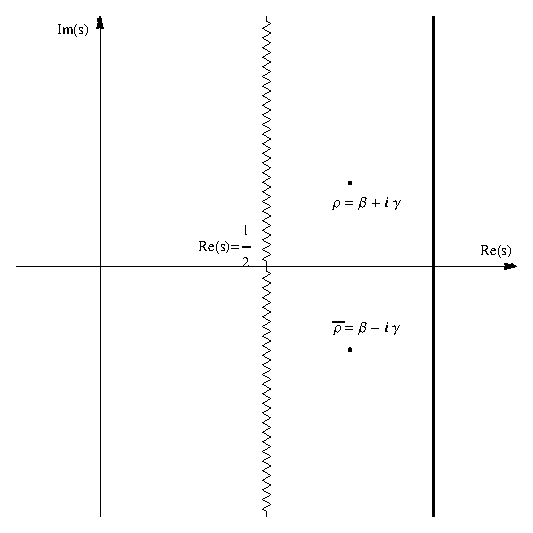
\includegraphics{ContoursPlots_gr2.eps}
	\caption{\textcolor{red}{Diagram explaining the bracketing process.}}
\end{figure}
\noindent These considerations now justify the bracketing condition for Dirichlet $L$-functions.
\begin{definition} \label{dirichlet_bracketing_condition}
Let us suppose that $A_1>0$ and $T>0$. Moreover, we let $T \to \infty$ through values such that $\left| {T - \gamma } \right| > \exp ( - A_1 \gamma /\log \gamma)$ for every ordinate $\gamma$ of a zero $\rho$ of $L(s,\chi)$. We define the bracketing condition $\mathcal{B}_\chi$ on a sum involving $\rho = \beta + i \gamma$ and $\rho' = \beta' + i \gamma'$ to be a summation where the terms are bracketed in such a way that two terms for which
\begin{align} \label{dirichlet_bracketing_condition_eq}
\left| {\gamma  - \gamma '} \right| < \exp ( - A_1 \gamma /\log \gamma ) + \exp ( - A_1 \gamma '/\log \gamma ')
\end{align}
are included in the same bracket. When a sum over $\rho$ satisfies the bracketing condition $\mathcal{B}_\chi$ we will write $\sum_{\rho \in \mathcal{B}}{f(\rho)}_\chi$.
\end{definition}
\noindent The following definition will restrict the class of functions to which $\varphi$ and $\psi$ might belong to.
\begin{definition}[\textcolor{red}{$\mathcal{K}$ class}]
\noindent If $\{\varphi, \psi \}$ is a pair of real-valued functions that satisfies the following conditions:
\begin{enumerate}
\item[\emph{1}]
\item[\emph{2}] ...
\end{enumerate}
then we say that $\{\varphi, \psi \}$ is in the class $\mathcal{K}$ and write $\{\varphi, \psi \} \in \mathcal{K}$.
\end{definition}
\noindent Finally, we will be needing the following results about Mellin transforms.
\begin{lemma}[\textcolor{red}{To be done}]
One has
\[\mathcal{M}(f(x),s) = O(\exp(-at + \varepsilon))\]
with $a>0$ and as $t \to \infty$.
\end{lemma}
%%%%%%%%%%%%%%%%%%%%%%%%%%%%%%%%%%%%%%%%%%%%%%%%%%%%%%%%%%%%%%%%%%%%%%%%%%%%%%%%%%%%%%%%%%%%%%%%%%%%%%%%%%%%%%%%%%%%%%%%%%%%%%%%%%%%%%%%%%%%%%%%%%%%%%
\subsection{Main result: Dirichlet $L$-functions}
\begin{theorem} \label{main_theorem}
Let $\varphi(x)$ and $\psi(x)$ be two functions in $\mathcal{K}$ and whose Mellin transforms are $Z_1(s)$ and $Z_2(s)$ respectively, furthermore let $\chi$ denote a primitive, even (odd) Dirichlet character of modulus $q$. If $a$ and $b$ are two positive reals such that $ab = \pi$ then one has
\begin{align} \label{main_theorem_eq}
  \sqrt a \sqrt {\tau (\chi )} \sum\limits_{n = 1}^\infty  {\frac{{\chi (n)\mu (n)}}
{n}\varphi \left( {\frac{a}
{{q^{1/2} n}}} \right)}  &- \sqrt b \sqrt {\tau (\bar \chi )} \sum\limits_{n = 1}^\infty  {\frac{{\bar \chi (n)\mu (n)}}
{n}\psi \left( {\frac{b}
{{q^{1/2} n}}} \right)}  \nonumber \\
   &= \frac{{q^{1/2} \sqrt {\tau (\chi )} }}
{{a^{1/2} }}\sum\limits_{\rho \in \mathcal{B}_\chi}  {\left( {\frac{a}
{{q^{1/2} }}} \right)^\rho  \frac{{\Gamma (1 - \rho )}}
{{L'(\rho ,\chi )}}Z_1 (1 - \rho )}  \nonumber \\
   &=  - \frac{{q^{1/2} \sqrt {\tau (\bar \chi )} }}
{{b^{1/2} }}\sum\limits_{\rho \in \mathcal{B}_\chi}  {\left( {\frac{b}
{{q^{1/2} }}} \right)^\rho  \frac{{\Gamma (1 - \rho )}}
{{L'(\rho ,\bar \chi )}}Z_2 (1 - \rho )}  \nonumber 
\end{align}
provided that the non-trivial zeros $\rho$ of $L(s,\chi)$ are all simple. 
\end{theorem}
\noindent To obtain Theorem \eqref{dixit} we consider different parities. If $\chi$ is even, then we take $\varphi (x) = \psi (x) = \exp ( - x^2 )$ which are cosine reciprocal. Thus,
\[
Z_1 (s) = Z_2 (s) = \frac{1}{{\Gamma (s)}}\Gamma \left( {\frac{s}{2}} \right)
\]
and the even case follows. On the other hand, if $\chi$ is odd then we take $\varphi (x) = \psi (x) = x\exp ( - x^2 )$ which are sine reciprocal. In this case,
\[
Z_1 (s) = Z_2 (s) = \frac{1}
{{\Gamma (s)}}\Gamma \left( {\frac{{1 + s}}
{2}} \right)
\]
and the odd case follows. In general, we are concerned with non-principal characters only so we have $q \ge 3$. However, if we let \textcolor{red}{$q \to 1$} then $\chi(n) = \bar \chi(n) =1$ for all $n$ and thus $L(s,\chi)=L(s,\bar \chi)=\zeta(s)$ as well as $\tau(\chi)=\tau(\bar \chi)=1$ and $\mathfrak{h}=0$ so that we obtain Theorem \eqref{ramanujan_generalization} as the limiting case.
\begin{proof}[Proof of Theorem \eqref{main_theorem}]
For $\sigma > 0$ and $-1 < \eta < 0$ we consider the positively oriented contour $\Omega = [\sigma - iT, \sigma + iT, \eta +iT, \eta-iT]$ where $T>0$ and $T \to \infty$. 
\begin{figure}[H]
	\centering
		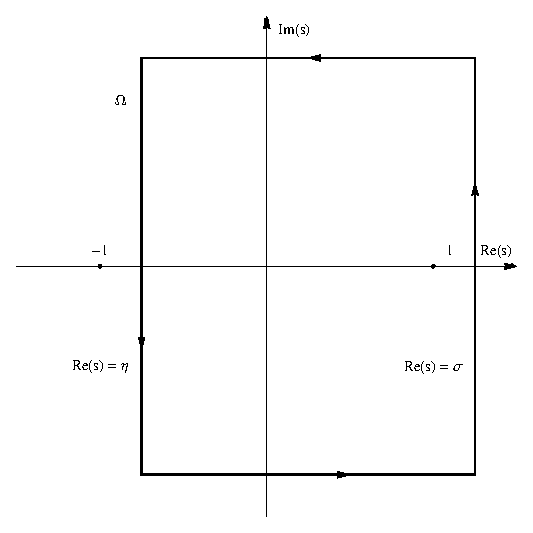
\includegraphics{ContoursPlots_gr3.eps}
	\caption{The contour $\Omega$.}
\end{figure}
\noindent Since $Z_k$ is analytic in this region and in particular at $s=0$ the residue theorem yields
\[
\frac{1}{{2\pi i}}\oint_\Omega  {x^{ - s} \Gamma (s)Z_k (s)ds}  = \mathop {\operatorname{res} }\limits_{s = 0} x^{ - s} \Gamma (s)Z_k (s) = Z_k (0).
\]
It will be shown \textcolor{red}{shortly} that the horizontal integrals $\tfrac{1}{{2\pi i}}\int_{\eta  - iT}^{\sigma  - iT}$ and $\tfrac{1}{{2\pi i}}\int_{\sigma  + iT}^{\eta  + iT}$ tend to zero as $T \to \infty$ so that we are left with
\begin{equation} \label{phi_psi_k_cases_eta}
\frac{1}
{{2\pi i}}\int_{\eta  - i\infty }^{\eta  + i\infty } {x^{ - s} \Gamma (s)Z_k (s)ds}  = \frac{1}
{{2\pi i}}\int_{\sigma  - i\infty }^{\sigma  + i\infty } {x^{ - s} \Gamma (s)Z_k (s)ds}  - Z_k(0) =
			\begin{cases}
{\varphi (x) - Z_1 (0)} & \mathrm{if\ } k=1, \\ 
{\psi (x) - Z_2 (0)} & \mathrm{if\ } k=2. 
			\end{cases}
\end{equation}
If $\chi$ is an even, primitive and non-principal character of modulus $q$ then $L(s,\chi)$ satisfies the functional equation
\[
\frac{1}{{L(1 - s,\chi )}} = \frac{{\tau (\bar \chi )}}{{q^{1/2} }}\left( {\frac{q}{\pi }} \right)^{1/2 - s} \frac{{\Gamma (\tfrac{{1 - s}}{2})}}{{\Gamma (\tfrac{s}{2})}}\frac{1}{{L(s,\bar \chi )}}.
\]
If we use the fact that $ab = \pi$ and couple this equation with the functional equation \eqref{FEcosine} of $Z_1$ and $Z_2$, we obtain
\begin{align} \label{FE_contour_integrals}
\frac{1}
{{2\pi i}}\oint_\Upsilon  {\left( {\frac{a}
{{q^{ 1/2} }}} \right)^{ - s} \frac{{\Gamma (s)}}
{{L(1 - s,\chi )}}Z_1 (s)ds}  = \frac{1}
{{2\pi i}}\oint_\Upsilon  {\frac{{\tau (\bar \chi )}}
{{\pi ^{1/2} }}\left( {\frac{b}
{{q^{1/2} }}} \right)^s \frac{{\Gamma (1 - s)}}
{{L(s,\bar \chi )}}Z_2 (1 - s)ds} 
\end{align}
where $\Upsilon$ is the positively oriented contour $[\lambda - iT, \lambda + iT, c+iT, c-iT]$ with $1< \lambda < \tfrac{5}{4}$ and $-1 < c < 0$. We denote by $\rho = \delta + i \gamma$ a non-trivial zero of $L(s,\bar \chi)$ and we choose $T>0$ to tend to infinity through values such that $|T - \gamma| > \exp(-A_1 \gamma / \log \gamma)$ for every ordinate $\gamma$ of a zero of $L(s,\bar \chi)$. By absolute convergence, with $c= \operatorname{Re}(s) < 0$, we may write
\begin{align}
  \frac{1}
{{2\pi i}}\int_{c - i\infty }^{c + i\infty } {\left( {\frac{a}
{{q^{1/2} }}} \right)^{ - s} \frac{{\Gamma (s)}}
{{L(1 - s,\chi )}}Z_1 (s)ds}  &= \frac{1}
{{2\pi i}}\int_{c - i\infty }^{c + i\infty } {\left( {\frac{a}
{{q^{1/2} }}} \right)^{ - s} \sum\limits_{n = 1}^\infty  {\frac{{\chi (n)\mu (n)}}
{{n^{1 - s} }}} \Gamma (s)Z_1 (s)ds}  \nonumber \\
   &= \sum\limits_{n = 1}^\infty  {\frac{{\chi (n)\mu (n)}}
{n}\frac{1}
{{2\pi i}}\int_{c - i\infty }^{c + i\infty } {\left( {\frac{a}
{{q^{1/2} n}}} \right)^{ - s} \Gamma (s)Z_1 (s)ds} }  \nonumber \\
   &= \sum\limits_{n = 1}^\infty  {\frac{{\chi (n)\mu (n)}}
{n}\varphi \left( {\frac{a}
{{q^{1/2} n}}} \right)}  - \frac{{Z_1 (0)}}
{{L(1,\chi )}} \nonumber 
\end{align}
where we have used the $k=1$ case of \eqref{phi_psi_k_cases_eta}. Similarly, with $\lambda = \operatorname{Re}(s) > 1$, we have
\begin{align}
  \frac{1}
{{2\pi i}}\int_{\lambda  - i\infty }^{\lambda  + i\infty } &{\frac{{\tau (\bar \chi )}}
{{\pi ^{1/2} }}\left( {\frac{b}
{{q^{1/2} }}} \right)^s \frac{{\Gamma (1 - s)}}
{{L(s,\bar \chi )}}Z_2 (1 - s)ds}  \nonumber \\
   &= \frac{1}
{{2\pi i}}\int_{\lambda  - i\infty }^{\lambda  + i\infty } {\frac{{\tau (\bar \chi )b^s }}
{{\pi ^{1/2} q^{s/2} }}\sum\limits_{n = 1}^\infty  {\frac{{\bar \chi (n)\mu (n)}}
{{n^s }}} \Gamma (1 - s)Z_2 (1 - s)ds}  \nonumber \\
   &= \frac{{\tau (\bar \chi )b}}
{{\pi ^{1/2} q^{1/2} }}\sum\limits_{n = 1}^\infty  {\frac{{\bar \chi (n)\mu (n)}}
{n}} \frac{1}
{{2\pi i}}\int_{1 - \lambda  - i\infty }^{1 - \lambda  + i\infty } {\left( {\frac{b}
{{q^{1/2} n}}} \right)^{ - w} \Gamma (w)Z_2 (w)dw}  \nonumber \\
   &= \frac{{\tau (\bar \chi )b}}
{{\pi ^{1/2} q^{1/2} }}\sum\limits_{n = 1}^\infty  {\frac{{\bar \chi (n)\mu (n)}}
{n}} \psi \left( {\frac{b}
{{q^{1/2} n}}} \right) - \frac{{\tau (\bar \chi )b}}
{{\pi ^{1/2} q^{1/2} }}\frac{{Z_2 (0)}}
{{L(1,\bar \chi )}} \nonumber 
\end{align}
by making the change $w=1-s$ and using the $k=2$ case of \eqref{phi_psi_k_cases_eta}. Now, we may use either side of \eqref{FE_contour_integrals} to evaluate the residues
\begin{itemize}
\item for the non-trivial zeros $\rho$ of $L(s,\chi)$, which we assume are all simple, we have
\[
\sum\limits_\rho  {\mathop {\operatorname{res} }\limits_{s = \rho } \frac{{\tau (\bar \chi )}}
{{\pi ^{1/2} }}\left( {\frac{b}
{{q^{1/2} }}} \right)^s \frac{{\Gamma (1 - s)}}
{{L(s,\bar \chi )}}Z_2 (1 - s)}  = \frac{{\tau (\bar \chi )}}
{{\pi ^{1/2} }}\sum\limits_\rho  {\left( {\frac{b}
{{q^{1/2} }}} \right)^\rho  \frac{{\Gamma (1 - \rho )}}
{{L'(\rho ,\bar \chi )}}Z_2 (1 - \rho )} 
\]
\item at $s=1$ we have a simple pole coming from the $\Gamma$ function
\[
\mathop {\operatorname{res} }\limits_{s = 1} \frac{{\tau (\bar \chi )}}
{{\pi ^{1/2} }}\left( {\frac{b}
{{q^{1/2} }}} \right)^s \frac{{\Gamma (1 - s)}}
{{L(s,\bar \chi )}}Z_2 (1 - s) =  - \frac{{\tau (\bar \chi )}}
{{\pi ^{1/2} }}\frac{b}
{{q^{1/2} }}\frac{{Z_2 (0)}}
{{L(1,\bar \chi )}}
\]
\item at $s=0$ we have a trivial (and simple) zero of $L(s,\bar \chi)$
\[
\mathop {\operatorname{res} }\limits_{s = 0} \frac{{\tau (\bar \chi )}}
{{\pi ^{1/2} }}\left( {\frac{b}
{{q^{1/2} }}} \right)^s \frac{{\Gamma (1 - s)}}
{{L(s,\bar \chi )}}Z_2 (1 - s) = \frac{{\tau (\bar \chi )}}
{{\pi ^{1/2} }}\frac{{Z_2 (1)}}
{{L'(0,\bar \chi )}} = \frac{{Z_1 (0)}}
{{L(1,\chi )}}
\]
\end{itemize}
where we have used Lemma \eqref{ABYC} with $q=N$ and $k=2$ in the last equality. Consequently, by the residue theorem we have
\[
\frac{{\tau (\bar \chi )b}}
{{\pi ^{1/2} q^{1/2} }}\sum\limits_{n = 1}^\infty  {\frac{{\bar \chi (n)\mu (n)}}
{n}\psi \left( {\frac{b}
{{q^{1/2} n}}} \right)}  - \sum\limits_{n = 1}^\infty  {\frac{{\chi (n)\mu (n)}}
{n}\varphi \left( {\frac{a}
{{q^{1/2} n}}} \right)}  = \frac{{\tau (\bar \chi )}}
{{\pi ^{1/2} }}\sum\limits_\rho  {\left( {\frac{b}
{{q^{1/2} }}} \right)^\rho  \frac{{\Gamma (1 - \rho )}}
{{L'(\rho ,\bar \chi )}}Z_2 (1 - \rho )} 
\]
Multiplying both sides by $- \sqrt a \sqrt {\tau (\chi )}$ and using the fact that $q^{1/2}  = \sqrt {\tau (\chi )\tau (\bar \chi )}$ we have the desired result for even characters
\begin{align}
& \sqrt a \sqrt {\tau (\chi )} \sum\limits_{n = 1}^\infty  {\frac{{\chi (n)\mu (n)}}
{n}\varphi \left( {\frac{a}
{{q^{1/2} n}}} \right)}  - \sqrt b \sqrt {\tau (\bar \chi )} \sum\limits_{n = 1}^\infty  {\frac{{\bar \chi (n)\mu (n)}}
{n}\psi \left( {\frac{b}
{{q^{1/2} n}}} \right)} \nonumber \\
&=  - q^{1/2} \frac{{\sqrt {\tau (\bar \chi )} }}
{{b^{1/2} }}\sum\limits_\rho  {\left( {\frac{b}
{{q^{1/2} }}} \right)^\rho  \frac{{\Gamma (1 - \rho )}}
{{L'(\rho ,\bar \chi )}}Z_2 (1 - \rho )}
\end{align}
We note that if we had used the other side of \eqref{FE_contour_integrals} instead, then the result would have been
\begin{align}
&\sqrt a \sqrt {\tau (\chi )} \sum\limits_{n = 1}^\infty  {\frac{{\chi (n)\mu (n)}}
{n}\varphi \left( {\frac{a}
{{q^{1/2} n}}} \right)}  - \sqrt b \sqrt {\tau (\bar \chi )} \sum\limits_{n = 1}^\infty  {\frac{{\bar \chi (n)\mu (n)}}
{n}\psi \left( {\frac{b}
{{q^{1/2} n}}} \right)} \nonumber \\
&= q^{1/2} \frac{{\sqrt {\tau ( \chi )} }}
{{a^{1/2} }}\sum\limits_\rho  {\left( {\frac{a}
{{q^{1/2} }}} \right)^\rho  \frac{{\Gamma (1 - \rho )}}
{{L'(\rho , \chi )}}Z_1 (1 - \rho )} 
\end{align}
To prove that the horizontal integrals tend to zero as $T \to \infty$ for the chosen values we note that from \eqref{angleLfunction} we obtain
\[
\frac{1}{{\left| {L(1 - s,\chi )} \right|}} < \exp (A_3 T)
\]
where $A_3 < \pi/2$. Using Stirling's formula
\[
\left| {\Gamma (s)} \right| = (2\pi )^{1/2} \left| t \right|^{\sigma  - 1/2} e^{ - \pi \left| t \right|/2} (1 + O(\left| t \right|^{ - 1} ))
\]
so that we have the bound
\[
\frac{1}
{{2\pi i}}\int_{\lambda  - iT}^{c - iT} {\left( {\frac{a}
{{q^{1/2} }}} \right)^{ - s} \frac{{\Gamma (s)}}
{{L(1 - s,\chi )}}Z_1 (s)ds}  = O\left( {T^{\sigma  - 1/2} \exp \left( {\left( {A_3  - \frac{\pi }
{2}} \right)T} \right)} \right)
\]
by the use of the \textcolor{red}{Mellin lemma}. The other horizontal integral is dealt with similarly. Let us now consider the case when $\chi$ is odd. For $\sigma > 0$ and $-1 < \eta < 0$ we consider the positively oriented contour $\Xi_\eta = [\sigma - iT, \sigma + iT, \eta +iT, \eta-iT]$ where $T>0$ and $T \to \infty$. Since $Z_k$ is analytic in this region and in particular at $s=0$ Cauchy theorem yields
\[
\frac{1}{{2\pi i}}\oint_{\Xi_\eta}  {x^{ - s} \Gamma (s)Z_k (s)ds}  = 0.
\]
Similarly as in the even case, it can be shown that the horizontal integrals $\tfrac{1}{{2\pi i}}\int_{\eta  - iT}^{\sigma  - iT}$ and $\tfrac{1}{{2\pi i}}\int_{\sigma  + iT}^{\eta  + iT}$ tend to zero as $T \to \infty$ so that we are left with
\begin{equation} \label{phi_psi_k_small_cases_eta_odd}
\frac{1}
{{2\pi i}}\int_{\eta  - i\infty }^{\eta  + i\infty } {x^{ - s} \Gamma (s)Z_k (s)ds}  = \frac{1}
{{2\pi i}}\int_{\sigma  - i\infty }^{\sigma  + i\infty } {x^{ - s} \Gamma (s)Z_k (s)ds}  =
			\begin{cases}
{\varphi (x)} & \mathrm{if\ } k=1, \\ 
{\psi (x)} & \mathrm{if\ } k=2. 
			\end{cases}
\end{equation}
For $- 2 < \theta  <  - 1$ we consider the positively oriented contour $\Xi_\theta = [\sigma - iT, \sigma + iT, \theta +iT, \theta-iT]$ where $T>0$ and $T \to \infty$. Since $Z_k$ is analytic in this region and in particular at $s=0$ the residue theorem yields
\[
\frac{1}
{{2\pi i}}\oint_{\Xi _\theta  } {x^{ - s} \Gamma (s)Z_k (s)ds}  = \mathop {\operatorname{res} }\limits_{s =  - 1} x^{ - s} \Gamma (s)Z_k (s) =  - xZ_k ( - 1)
\]
Again, the horizontal integrals will tend to zero as $T \to \infty$ so that we have
\begin{equation} \label{phi_psi_k_largel_cases_eta_odd}
\frac{1}
{{2\pi i}}\int_{\theta  - iT}^{\theta  + iT} {x^{ - s} \Gamma (s)Z_k (s)ds} = 
			\begin{cases}
{\varphi (x) + xZ_1(-1)} & \mathrm{if\ } k=1, \\ 
{\psi (x) + xZ_2(-1)} & \mathrm{if\ } k=2. 
			\end{cases}
\end{equation}
If $\chi$ is an odd, primitive and non-principal character of modulus $q$ then $L(s,\chi)$ satisfies the functional equation
\[
\frac{1}
{{L(1 - s,\chi )}} = \frac{{\tau (\bar \chi )}}
{{iq^{1/2} }}\left( {\frac{q}
{\pi }} \right)^{1/2 - s} \frac{{\Gamma (1 - \tfrac{s}
{2})}}
{{\Gamma (\tfrac{{s + 1}}
{2})}}\frac{1}
{{L(s,\bar \chi )}}
\]
If we use the fact that $ab = \pi$ and couple this equation with the functional equation \eqref{FEsine} of $Z_1$ and $Z_2$, we obtain
\[
\frac{1}
{{2\pi i}}\oint_\Psi  {\left( {\frac{a}
{{q^{1/2} }}} \right)^{ - s} \frac{{\Gamma (s)}}
{{L(1 - s,\chi )}}Z_1 (s)ds}  = \frac{1}
{{2\pi i}}\oint_\Psi  {\frac{{\tau (\bar \chi )}}
{{i\pi ^{1/2} }}\left( {\frac{b}
{{q^{1/2} }}} \right)^s \frac{{\Gamma (1 - s)}}
{{L(s,\bar \chi )}}Z_2 (1 - s)ds} 
\]
where $\Psi  = [\lambda  - iT,\lambda  + iT,\theta  + iT,\theta  - iT]$ with $1 < \lambda  < \tfrac{3}{2}$. By absolute convergence with $\operatorname{Re}(s) = \theta$ we can change summation and integration to obtain
\begin{align}
  \frac{1}
{{2\pi i}}\int_{\theta  - i\infty }^{\theta  + i\infty } {\left( {\frac{a}
{{q^{1/2} }}} \right)^{ - s} \frac{{\Gamma (s)}}
{{L(1 - s,\chi )}}Z_1 (s)ds} &= \frac{1}
{{2\pi i}}\int_{\theta  - i\infty }^{\theta  + i\infty } {\left( {\frac{a}
{{q^{1/2} }}} \right)^{ - s} \sum\limits_{n = 1}^\infty  {\frac{{\chi (n)\mu (n)}}
{{n^{1 - s} }}} \Gamma (s)Z_1 (s)ds}  \nonumber \\
   &= \sum\limits_{n = 1}^\infty  {\frac{{\chi (n)\mu (n)}}
{n}\frac{1}
{{2\pi i}}\int_{\theta  - i\infty }^{\theta  + i\infty } {\left( {\frac{a}
{{q^{1/2} n}}} \right)^{ - s} \Gamma (s)Z_1 (s)ds} }  \nonumber \\
   &= \sum\limits_{n = 1}^\infty  {\frac{{\chi (n)\mu (n)}}
{n}\varphi \left( {\frac{a}
{{q^{1/2} n}}} \right)}  + \frac{{aZ_1 ( - 1)}}
{{q^{1/2} L(2,\chi )}} 
\end{align}
Moreover, also by absolute convergence with $\operatorname{Re}(s) = \lambda$, we have
\begin{align}
  \frac{1}
{{2\pi i}}\int_{\lambda  - i\infty }^{\lambda  + i\infty } {\frac{{\tau (\bar \chi )}}
{{i\pi ^{1/2} }}\left( {\frac{b}
{{q^{1/2} }}} \right)^s \frac{{\Gamma (1 - s)}}
{{L(s,\bar \chi )}}Z_2 (1 - s)ds} &= \frac{{\tau (\bar \chi )}}
{{i\pi ^{1/2} }}\frac{1}
{{2\pi i}}\int_{\lambda  - i\infty }^{\lambda  + i\infty } {\left( {\frac{b}
{{q^{1/2} }}} \right)^s }  \nonumber \\
   &\times \sum\limits_{n = 1}^\infty  {\frac{{\bar \chi (n)\mu (n)}}
{{n^s }}} \Gamma (1 - s)Z_2 (1 - s)ds \nonumber \\
%   &= \frac{{\tau (\bar \chi )}}
%{{i\pi ^{1/2} }}\sum\limits_{n = 1}^\infty  {\bar \chi (n)\mu (n)\frac{1}
%{{2\pi i}}\int_{\lambda  - i\infty }^{\lambda  + i\infty } {\left( {\frac{b}
%{{q^{1/2} n}}} \right)^s \Gamma (1 - s)Z_2 (1 - s)ds} }  \nonumber \\
   &= \frac{{\tau (\bar \chi )}}
{{i\pi ^{1/2} }}\frac{b}
{{q^{1/2} }}\sum\limits_{n = 1}^\infty  {\frac{{\bar \chi (n)\mu (n)}}
{n}}  \nonumber \\
   &\times \frac{1}
{{2\pi i}}\int_{1 - \lambda  - i\infty }^{1 - \lambda  + i\infty } {\left( {\frac{b}
{{q^{1/2} n}}} \right)^{ - w} \Gamma (w)Z_2 (w)dw}  \nonumber \\
   &= \frac{{\tau (\bar \chi )}}
{{i\pi ^{1/2} }}\frac{b}
{{q^{1/2} }}\sum\limits_{n = 1}^\infty  {\frac{{\bar \chi (n)\mu (n)}}
{n}\psi \left( {\frac{b}
{{q^{1/2} n}}} \right)} 
\end{align}
where we have made the change $w=1-s$. By the \textcolor{red}{Mellin lemma}, we know that the contribution from the horizontal integrals of this contour will tend to zero. Next, we compute the residues
\begin{itemize}
\item for the non-trivial zeros $\rho$ one has
\[
\sum\limits_\rho  {\mathop {\operatorname{res} }\limits_{s = \rho } \frac{{\tau (\bar \chi )}}
{{i\pi ^{1/2} }}\left( {\frac{b}
{{q^{1/2} }}} \right)^s \frac{{\Gamma (1 - s)}}
{{L(s,\bar \chi )}}Z_2 (1 - s)}  = \frac{{\tau (\bar \chi )}}
{{i\pi ^{1/2} }}\sum\limits_\rho  {\left( {\frac{b}
{{q^{1/2} }}} \right)^\rho  \frac{{\Gamma (1 - \rho )}}
{{L'(\rho ,\bar \chi )}}Z_2 (1 - \rho )} 
\]
\item for the trivial zero of $L(s,\bar \chi)$ at $s=-1$ one has
\begin{align}
\mathop {\operatorname{res} }\limits_{s =  - 1} \frac{{\tau (\bar \chi )}}
{{i\pi ^{1/2} }}\left( {\frac{b}
{{q^{1/2} }}} \right)^s \frac{{\Gamma (1 - s)}}
{{L(s,\bar \chi )}}Z_2 (1 - s) &= \frac{{\tau (\bar \chi )}}
{{i\pi ^{1/2} }}\frac{{q^{1/2} }}
{b}\frac{{Z_2 (2)}}
{{L'( - 1,\bar \chi )}} = \frac{1}
{b}Z_2 (2)\frac{{4\pi ^{1/2} }}
{{q^{1/2} }}\frac{1}
{{L(2,\chi )}} \nonumber \\
&=  - \frac{a}
{{q^{1/2} }}\frac{{Z_1 ( - 1)}}
{{L(2,\chi )}}
\end{align}
\end{itemize}
where we have used the Lemma \eqref{ABYC} with $q=N$ and $k=3$. By the residue theorem one has
\begin{align}
  &\frac{{\tau (\bar \chi )}}
{{i\pi ^{1/2} }}\frac{b}
{{q^{1/2} }}\sum\limits_{n = 1}^\infty  {\frac{{\bar \chi (n)\mu (n)}}
{n}\psi \left( {\frac{b}
{{q^{1/2} n}}} \right)}  - \sum\limits_{n = 1}^\infty  {\frac{{\chi (n)\mu (n)}}
{n}\varphi \left( {\frac{a}
{{q^{1/2} n}}} \right)}  - \frac{{aZ_1 ( - 1)}}
{{q^{1/2} L(2,\chi )}} \nonumber \\
   &= \frac{{\tau (\bar \chi )}}
{{i\pi ^{1/2} }}\sum\limits_\rho  {\left( {\frac{b}
{{q^{1/2} }}} \right)^\rho  \frac{{\Gamma (1 - \rho )}}
{{L'(\rho ,\bar \chi )}}Z_2 (1 - \rho )}  - \frac{a}
{{q^{1/2} }}\frac{{Z_1 ( - 1)}}
{{L(2,\chi )}} \nonumber 
\end{align}
Multiplying by $-\sqrt a \sqrt {\tau (\chi )}$ and using the fact that $\sqrt{\tau(\chi) \tau(\bar \chi)} = i q^{1/2}$ one has
\begin{align}
  &\sqrt a \sqrt {\tau (\chi )} \sum\limits_{n = 1}^\infty  {\frac{{\chi (n)\mu (n)}}
{n}\varphi \left( {\frac{a}
{{q^{1/2} n}}} \right)}  - \sqrt b \sqrt {\tau (\bar \chi )} \sum\limits_{n = 1}^\infty  {\frac{{\bar \chi (n)\mu (n)}}
{n}\psi \left( {\frac{b}
{{q^{1/2} n}}} \right)}  \nonumber \\
 &  =  - \frac{{q^{1/2} }}
{{b^{1/2} }}\sqrt {\tau (\bar \chi )} \sum\limits_\rho  {\left( {\frac{b}
{{q^{1/2} }}} \right)^\rho  \frac{{\Gamma (1 - \rho )}}
{{L'(\rho ,\bar \chi )}}Z_2 (1 - \rho )}
\end{align}
and this proves the theorem.
\end{proof}
%%%%%%%%%%%%%%%%%%%%%%%%%%%%%%%%%%%%%%%%%%%%%%%%%%%%%%%%%%%%%%%%%%%%%%%%%%%%%%%%%%%%%%%%%%%%%%%%%%%%%%%%%%%%%%%%%%%%%%%%%%%%%%%%%%%%%%%%%%%%%%%%%%%%%%
%%%%%%%%%%%%%%%%%%%%%%%%%%%%%%%%%%%%%%%%%%%%%%%%%%%%%%%%%%%%%%%%%%%%%%%%%%%%%%%%%%%%%%%%%%%%%%%%%%%%%%%%%%%%%%%%%%%%%%%%%%%%%%%%%%%%%%%%%%%%%%%%%%%%%%
\section{Criteria for the Riemann hypothesis}
\noindent Let us suppose that $\varphi(x)$ and $\psi(x)$ are in the class $\mathcal{K}$ and $q=1$. For $y>0$, let us define the functions
\[{P_\varphi }(y): = \sum\limits_{n = 1}^\infty  {\frac{{\mu (n)}}{n}\varphi \left( {\frac{y}{n}} \right)} ,\quad {P_\psi }(y): = \sum\limits_{n = 1}^\infty  {\frac{{\mu (n)}}{n}\psi \left( {\frac{y}{n}} \right)}. \]
Now we perform a Maclaurin expansion of $\varphi$ around $y=0$ to obtain
\[{P_\varphi }(y) = \sum\limits_{n = 1}^\infty  {\frac{{\mu (n)}}{n}\sum\limits_{k = 0}^\infty  {{{\left( {\frac{y}{n}} \right)}^k}} \frac{{{\varphi ^{(k)}}(0)}}{{k!}}}  = \sum\limits_{k = 0}^\infty  {\frac{{{\varphi ^{(k)}}(0)}}{{k!}}{y^k}\sum\limits_{n = 1}^\infty  {\frac{{\mu (n)}}{{{n^{k + 1}}}}} }  = \sum\limits_{k = 0}^\infty  {\frac{{{\varphi ^{(k)}}(0)}}{{k!}}\frac{{{y^k}}}{{\zeta (1 + k)}}}, \]
with a similar formula holding for ${P_\psi }(y)$. The explicit formula of Hardy, Littlewood and Ramanujan may be written as
\begin{align} \label{explicit_P}
{a^{\tfrac{1}{2}}}{P_\varphi }(a) - {b^{\tfrac{1}{2}}}{P_\psi }(b) =  -\sum\limits_\rho  {{b^{\rho -\tfrac{1}{2}}}\frac{{\Gamma (1 - \rho )}}{{\zeta '(\rho )}}{Z_2}(1 - \rho )}.
\end{align}
If we assume the Riemann hypothesis, $\rho= \tfrac{1}{2} + i \gamma$ with $\gamma \in \R$, and the absolute convergence of
\[\sum\limits_\rho  {\frac{{\Gamma (1 - \rho )}}{{\zeta '(\rho )}}{Z_2}(1 - \rho )}, \]
then the right-hand side of \eqref{explicit_P} is of the form $O(1)$ when $a \to 0^+$ and $b \to \infty$. Also, by the prime number theorem, the first term on the left-hand side of \eqref{explicit_P} becomes
\[{a^{\tfrac{1}{2}}}{P_\varphi }(a) = {a^{\tfrac{1}{2}}}\sum\limits_{n = 1}^\infty  {\frac{{\mu (n)}}{n}\varphi \left( {\frac{a}{n}} \right)}  = {a^{\tfrac{1}{2}}}\sum\limits_{n = 1}^\infty  {\frac{{\mu (n)}}{n}O(1)}  = 0,\]
since $\varphi(a) = O(1)$ as $a \to 0^+$. Thus the remaining term is now $- {b^{\tfrac{1}{2}}}{P_\psi}(b) = O(1)$, or, equivalently
\begin{align} \label{boundonPtaylor}
\sum\limits_{k = 0}^\infty  {\frac{{{\psi ^{(k)}}(0)}}{{k!}}\frac{{{b^k}}}{{\zeta (1 + k)}}}  = O({b^{ - \tfrac{1}{2}}}),
\end{align}
as $b \to \infty$. Seeing how the Riemann hypothesis implies the bound \eqref{boundonPtaylor}, we will now establish that the converse is also true as well as remove the assumption on the absolute convergence of the sum involving the zeros.
\begin{theorem}
Let us suppose that $\varphi(x)$ and $\psi(x)$ are in the class $\mathcal{K}$ and consider the function
\[{P_\varphi }(y): = \sum\limits_{k = 0}^\infty  {\frac{{{\varphi ^{(k)}}(0)}}{{k!}}\frac{{{y^k}}}{{\zeta (1 + k)}}} .\]
One has the following:
\begin{enumerate}
\item[\emph{i}] The Riemann hypothesis implies $P_\varphi(y) = O({y^{ - \tfrac{1}{2} + \delta }})$ as $y \to \infty$ for all $\delta >0$.
\item[\emph{ii.a}] If $Z_1(-s)$ has no zeros in the interval $-\tfrac{1}{2} < \real(s) \le 0$, then the estimate $P_\varphi(y) = O({y^{ - \tfrac{1}{2} + \delta }})$ as $y \to \infty$ for all $\delta >0$ implies the Riemann hypothesis.
\item[\emph{ii.b}] If $Z_1(s)$ has zeros in the interval $-\tfrac{1}{2} < \real(s) \le 0$, then the estimate $P_\varphi(y) = O({y^{ - \tfrac{1}{2} + \delta }})$ as $y \to \infty$ for all $\delta >0$ implies that $\zeta(s)$ has at most finitely many non-trivial zeros off the critical line.
\end{enumerate}
\end{theorem}
\begin{proof}
\noindent For $0<c<1$ we define
\[W(x): = \frac{1}{{2\pi i}}\int_{c - i\infty }^{c + i\infty } {\frac{{\Gamma ( - s){Z_1}( - s)}}{{\zeta (1 + s)}}{x^s}ds}. \]
By using the fact that $c>0$ we can write
\[W(x) = \frac{1}{{2\pi i}}\int_{c - i\infty }^{c + i\infty } {\Gamma ( - s){Z_1}( - s)\sum\limits_{n = 1}^\infty  {\frac{{\mu (n)}}{{{n^{1 + s}}}}} {x^s}ds}  = \sum\limits_{n = 1}^\infty  {\frac{{\mu (n)}}{n}\frac{1}{{2\pi i}}\int_{c - i\infty }^{c + i\infty } {\Gamma ( - s){Z_1}( - s){{\left( {\frac{n}{x}} \right)}^{ - s}}ds} }. \]
The change of variable $w=-s$ yields
\begin{align}
  W(x) &= \sum\limits_{n = 1}^\infty  {\frac{{\mu (n)}}{n}\frac{1}{{2\pi i}}\int_{ - c - i\infty }^{ - c + i\infty } {\Gamma (w){Z_1}(w){{\left( {\frac{x}{n}} \right)}^{ - w}}dw} }  \nonumber \\
   &= \sum\limits_{n = 1}^\infty  {\frac{{\mu (n)}}{n}\left\{ {\varphi \left( {\frac{x}{n}} \right) - \mathop {\operatorname{res} }\limits_{w = 0} \Gamma (w){Z_1}(w){{\left( {\frac{x}{n}} \right)}^{ - w}}} \right\}}  = \sum\limits_{n = 1}^\infty  {\frac{{\mu (n)}}{n}\left\{ {\varphi \left( {\frac{x}{n}} \right) - {Z_1}(0)} \right\}}  \nonumber \\
   &= \sum\limits_{n = 1}^\infty  {\frac{{\mu (n)}}{n}\varphi \left( {\frac{x}{n}} \right)}  = {P_\varphi }(x), \nonumber 
\end{align}
where in the first equality of the second line we have used the fact that $- 1 <  - c < 0$ and the prime number theorem on the third line. We apply a Mellin inversion to obtain
\[\Phi (s): = \int_0^\infty  {{P_\varphi }(x){x^{ - s - 1}}dx}  = \frac{{\Gamma ( - s){Z_1}( - s)}}{{\zeta (1 + s)}}.\]
Therefore, multiplying both sides by $s$ we have that 
\begin{align} \label{deductionRH}
{s\zeta (1 + s)\Phi (s) = \Gamma (1 - s){Z_1}( - s)},
\end{align}
for $0 < \operatorname{Re} (s) < 1$. Next, we split the integral representation of $\varphi(s)$ and apply the bound ${P_\varphi }(x) = O({x^{ - \tfrac{1}{2} + \delta }})$ for any $\delta >0$ as $x \to \infty$ and for all suitable $\varphi$ so that
\begin{align}
  \Phi (s) & = \int_0^1 {{P_\varphi }(x){x^{ - s - 1}}dx}  + \int_1^\infty  {{P_\varphi }(x){x^{ - s - 1}}dx}  \nonumber \\
   &= \int_0^1 {O({x^{\tfrac{1}{2} - \delta }}){x^{ - s - 1}}dx}  + \int_1^\infty  {O({x^{ - \tfrac{1}{2} + \delta }}){x^{ - s - 1}}dx}  \nonumber \\
   &\ll \frac{2}{{1 + 2s - 2\delta }} - \frac{2}{{ - 1 + 2s + 2\delta }} \nonumber \\
   &= \frac{{4 - 8\delta }}{{{{(1 - 2\delta )}^2} - 4{s^2}}}, \nonumber 
\end{align}
provided that
\[\operatorname{Re} (s) - \delta  >  - \frac{1}{2}.\]
Thus one can now see that the application of the bound ${P_\varphi }(x) = O({x^{ - \tfrac{1}{2} + \delta }})$ makes the integral analytic on the interval $-\tfrac{1}{2} < \real(s) \le 0$. We now reason as follows. Since the simple pole of $\zeta(1-s)$ is annihilated by the zero of $s$ at $s=0$ we see that the left-hand side of \eqref{deductionRH} is analytic. Moreover, since $\Gamma(1-s)$ does not have any poles in $-\tfrac{1}{2} < \real(s) \le 0$ and $Z_1(s)$ is analytic\footnote{To be checked} in $-\tfrac{1}{2} < \real(s) \le 0$, the right-hand side of \eqref{deductionRH} is also analytic on $-\tfrac{1}{2} < \real(s) \le 0$. Since \eqref{deductionRH} holds for $0 < \real(s) < 1$, by the theory of analytic continuation, it holds on $-\tfrac{1}{2} < \real(s) \le 0$. Next, since $\Gamma(1-s)$ does not have any zeros, the zeros of the right-hand side of \eqref{deductionRH} are the zeros of $Z_1(-s)$. We now distinguish two cases.
\begin{enumerate}
\item If $Z_1(-s)$ does not have any zeros in the interval $-\tfrac{1}{2} < \real(s) \le 0$, then the left-hand side of \eqref{deductionRH} is non-zero in $-\tfrac{1}{2} < \real(s) \le 0$. However, since $\Phi(s)$ has been shown to be analytic in this interval when the bound on $P_\varphi(x)$ is applied, this implies that $\zeta(1+s)$ does not have zeros in $-\tfrac{1}{2} < \real(s) \le 0$. This implies the Riemann hypothesis.
\item If $Z_1(-s)$ does have zeros in the interval $-\tfrac{1}{2} < \real(s) \le 0$, then because $Z_1(s)$ is entire, it must be a finite number of zeros in any truncated region of this interval. By Stirling's formula, we also see that\footnote{This needs to be cleaned up. Also, it shows that $Z_1(s)$ has a simple pole at $s=1$, before applying the functional equation. Perhaps this should be in the lemma regarding the functional equation of $Z_1(s)$ etc.} for $\real(s)>0$ one has
\begin{align} \label{whynofluctuation}
  {Z_1}(s) &= \frac{1}{{\Gamma (s)}}\int_0^\infty  {{x^{s - 1}}\varphi (x)dx}  = \frac{1}{{\Gamma (s)}}\int_0^1 {{x^{s - 1}}\varphi (x)dx}  + \frac{1}{{\Gamma (s)}}\int_1^\infty  {{x^{s - 1}}\varphi (x)dx}  \nonumber \\
   &\ll  {\frac{1}{{s\Gamma (s)}}}  +  {\frac{1}{{(1 - s)\Gamma (s)}}} ,\quad (0 < \operatorname{Re} (s) < 1) \nonumber \\
   &=  {\frac{1}{{\Gamma (s)}}\left( {\frac{1}{s} + \frac{1}{{1 - s}}} \right)} ,\quad (\operatorname{Re} (s) \ne 1) \nonumber \\
   &\sim \frac{1}{{\sqrt {2\pi } }}\exp \left( {\frac{1}{2}\pi \left| t \right|} \right){\left| t \right|^{ - \sigma  + \tfrac{1}{2}-2}} \\
   &\to \infty  \nonumber 
\end{align}
for $\sigma \in \R\backslash\{1\}$ and as $t \to \infty$. This also shows that $Z_1(-s)$ tends to $\infty$ as $t \to \infty$. This means that for fixed $\sigma$ in the interval $-\tfrac{1}{2} < \real(s) \le 0$ and as $t$ grows, the function $Z_1(-s)$ tends to infinity in absolute value as $\left| s \right| \to \infty$, implying that for $t$ large enough, we have $\left| {{Z_1}(-s)} \right| > 0$. Thus, there exists a $T_0$ such that for all $t > T_0$ we have ${Z_1}(-s) \ne 0$. Consequently, the left-hand side of \eqref{deductionRH} has zeros at most up to a fixed height $t_0$, depending on the choice of $\varphi(x)$. However, we also know that $\zeta(s)$ has only finitely many zeros up to a fixed height $t_0$.\\
This means that (a) the estimate ${P_\varphi }(y) = O({y^{\tfrac{1}{2} + \delta }})$ as $y \to \infty$ for all $\delta >0$ and, (b) the fact that $Z_1(-s)$ has finitely many zeros, imply that $\zeta(s)$ has at most finitely many non-trivial zeros off the critical line. The number of such zeros will be linked to the number of zeros of $Z_1(-s)$.
\end{enumerate}
\noindent Let us now prove that the Riemann hypothesis implies the bound ${P_\varphi }(y) = O({y^{\tfrac{1}{2} + \delta }})$ as $y \to \infty$ for all $\delta >0$. One formulation of the Riemann hypothesis involving Merten's function $M(x): = \sum\nolimits_{n \leqslant x} {\mu (n)}$ is that $M(x) = {O_\varepsilon }({x^{\tfrac{1}{2} + \varepsilon }})$ as $x \to \infty$ for all $\varepsilon >0$. An application of partial summation allows us to transform this into
\begin{align} \label{RH_mertens_partial}
M(\nu ,n): = \sum\limits_{m = \nu }^n {\frac{{\mu (m)}}{m}}  = {O_\varepsilon }({\nu ^{ - \tfrac{1}{2} + \varepsilon }})
\end{align}
uniformly in $n$. Recalling the definition of $P_\varphi$ we have
\[{P_\varphi }(y) = \sum\limits_{n = 1}^\infty  {\frac{{\mu (n)}}{n}\varphi \left( {\frac{y}{n}} \right)}  = \left[ {\sum\limits_{n = 1}^{\nu  - 1} {}  + \sum\limits_{n = \nu }^\infty  {} } \right]\frac{{\mu (n)}}{n}\varphi \left( {\frac{y}{n}} \right) = :{P_{\varphi ,1}}(y) + {P_{\varphi ,2}}(y),\]
say, where $\nu  = [{y^{1 - \varepsilon }}]$. For the first sum we have
\[{P_{\varphi ,1}}(y) = \sum\limits_{n = 1}^\nu  {\frac{{\mu (n)}}{n}\varphi \left( {\frac{y}{n}} \right)}  = \sum\limits_{n = 1}^\nu  {M(\nu ,n)\left\{ {\varphi \left( {\frac{y}{n}} \right) - \varphi \left( {\frac{y}{{n + 1}}} \right)} \right\}}  = O\left( {\sum\limits_{n = 1}^\nu  {M(\nu ,n)} } \right).\]
If we now use \eqref{RH_mertens_partial} in the above, we then obtain
\begin{align}
  {P_{\varphi ,1}}(y) &= O\left( {\sum\limits_{n = 1}^\nu  {{O_\varepsilon }({\nu ^{ - \tfrac{1}{2} + \varepsilon }})} } \right) = {O_\varepsilon }\left( {{\nu ^{ - \tfrac{1}{2} + \varepsilon }}\sum\limits_{n = 1}^\nu  1 } \right) = {O_\varepsilon }({\nu ^{\tfrac{1}{2} + \varepsilon }}) \nonumber \\
   &= {O_\varepsilon }({({y^{1 - \varepsilon }})^{\tfrac{1}{2} + \varepsilon }}) = {O_\varepsilon }({y^{\tfrac{1}{2} + \tfrac{\varepsilon }{2} - {\varepsilon ^2}}}) = {O_\varepsilon }({y^{\tfrac{1}{2} + \varepsilon }}). \nonumber 
\end{align}
For the second sum, we have
\begin{align}
  {P_{\varphi ,2}}(y) &= \sum\limits_{n = \nu }^\infty  {\frac{{\mu (n)}}{n}\varphi \left( {\frac{y}{n}} \right)}  = \sum\limits_{n = \nu }^\infty  {M(\nu ,n)\left\{ {\varphi \left( {\frac{y}{n}} \right) - \varphi \left( {\frac{y}{{n + 1}}} \right)} \right\}}  \nonumber \\
   &= \sum\limits_{n = \nu }^\infty  {M(\nu ,n)\left\{ { - \frac{y}{{\lambda _n^2}}\varphi '\left( {\frac{y}{{{\lambda _n}}}} \right)} \right\}},  \nonumber 
\end{align}
where in the last line we have used the mean value theorem with $a=n < \lambda_n (=c) < n+1=b$. Noting that $\varphi'(x)$ is $O(1)$ as $x \to 0^+$ yields
\begin{align}
  {P_{\varphi ,2}}(y)  &=  - y\sum\limits_{n = \nu }^\infty  {M(\nu ,n)\left\{ {\frac{1}{{\lambda _n^2}}\varphi '\left( {\frac{y}{{{\lambda _n}}}} \right)} \right\}}  = O\left( {y\sum\limits_{n = \nu }^\infty  {M(\nu ,n)\frac{1}{{\lambda _n^2}}} } \right) \nonumber \\
   &= O\left( {y\sum\limits_{n = \nu }^\infty  {{O_\varepsilon }({\nu ^{ - \tfrac{1}{2} + \varepsilon }})\frac{1}{{\lambda _n^2}}} } \right) = {O_\varepsilon }\left( {y{\nu ^{ - \tfrac{1}{2} + \varepsilon }}\sum\limits_{n = \nu }^\infty  {\frac{1}{{\lambda _n^2}}} } \right) \nonumber \\
   &= {O_\varepsilon }\left( {y{{({y^{1 - \varepsilon }})}^{ - \tfrac{1}{2} + \varepsilon }}\sum\limits_{n = \nu }^\infty  {\frac{1}{{\lambda _n^2}}} } \right) = {O_\varepsilon }(y \cdot {y^{ - \tfrac{1}{2} + \varepsilon  + \tfrac{1}{2}\varepsilon  - {\varepsilon ^2}}}O(1)) \nonumber \\
   &= {O_\varepsilon }({y^{\tfrac{1}{2} + \tfrac{3}{2}\varepsilon  - {\varepsilon ^2}}}) = {O_\varepsilon }({y^{\tfrac{1}{2} + \varepsilon }}). \nonumber 
\end{align}
This means that the Riemann hypothesis implies the bound ${P_\varphi }(y) = O({y^{\tfrac{1}{2} + \delta }})$ as $y \to \infty$ for all $\delta >0$ as it was to be shown.
\end{proof}
\noindent Let us now go back to $\Phi (s)$. We have shown that for $0< \real(s) < 1$ one has
\begin{align} \label{deductionFEPhi}
\zeta (1 + s)\Phi (s) = \Gamma ( - s){Z_1}( - s).
\end{align}
We know that $Z_1(-s)$ has simple zeros at $1,3,5,\cdots$ and that $\Gamma(-s)$ has simple poles at $s=0,1,2,3,\cdots$. Thus, the simple poles on the right-hand side of \eqref{deductionFEPhi} at $s=0,2,4,6,\cdots$ have to be accounted for on the left-hand side. For $s=0$, we know that $\zeta(1+s)$ has a simple pole thus $\Phi(s)$ is regular at $s=0$. However, this means that $\Phi(s)$ has simple poles at $s=2,4,6,\cdots$. Moreover, $\zeta(1+s)$ has simple zeros at $s=-1,-3,-5,\cdots$ therefore either
\begin{enumerate}
\item[1a.] $\Phi(s)$ has simple poles at $s=-1,-3,-5,\cdots$, or
\item[1b.] $Z_1(-s)$ has simple zeros at $s=-1,-3,-5,\cdots$.
\end{enumerate}
Likewise for the non-trivial zeros $s=\rho-1$, i.e. either
\begin{enumerate}
\item[2a.] $\Phi(s)$ has poles of unknown order at $s=\rho-1$, or
\item[2b.] $Z_1(-s)$ has zeros of unknown order at $s=\rho-1$.
\end{enumerate}
Furthermore, let us say that $Z_1(s)$ has \textit{additional} zeros at $s=s_1,s_2,s_3,\cdots$ so that $Z_1(-s)$ has zeros at $s=-s_1,-s_2,-s_3,\cdots$. This would mean that either $\zeta(1+s)$ or $\Phi(s)$ would have to vanish at $s=-s_1,-s_2,-s_3,\cdots$. It couldn't possibly\footnote{To be shown or explained!} be $\zeta(1+s)$, so if additional zeros of $Z_1(-s)$ exist then $\Phi(s)$ would have to vanish at those zeros as well.\\
By the use of the functional equation of the Riemann zeta-function we have
\[\zeta ( - s)\Phi (s) = {2^{ - (1 + s)}}{\pi ^{ - s}}\sec \left( {\frac{{\pi s}}{2}} \right){Z_1}( - s),\]
whereas if we apply the functional equations of $\zeta(s)$ and of $Z_1(s)$, then \eqref{deductionFEPhi} can alternatively be written in terms of the function $Z_2$ as
\[\zeta ( - s)\Phi (s) = {\pi ^{ - s - \tfrac{1}{2}}}\Gamma (s + 1){Z_2}(s + 1).\]
If we combine the above then we obtain the rather unsymmetrical functional equation
\[{\pi ^{(s - 1)/2}}{Z_1}( - s)\zeta (s - 1)\Phi (1 - s) = {\pi ^{\tfrac{s}{2} - 1}}{Z_2}( - s)\zeta (s + 1)\Phi (s).\]
Let us now illustrate a specific example. It is now that up to height $T$, the number of zeros of $\zeta(s)$ is given by the Riemann-von Mangoldt formula
\[N(T) = \frac{T}{{2\pi }}\log \frac{T}{{2\pi }} - \frac{T}{{2\pi }} + O(\log T).\]
Dixit, Roy and Zaharescu have considered the special cases where $\varphi (x) = {e^{ - {x^2}}}\cosh (xz)$ and where $\psi (x) = {e^{ - {x^2}}}\cos (xz)e^{-z^2/4}$ with $z \in \C$ fixed. The Mellin transform is this case is given by
\[{Z_{1,2}}(s) = {\frac{{\Gamma (\tfrac{s}{2})}}{{2\Gamma (s)}}}{_1F_1}\left( {\frac{s}{2},\frac{1}{2}, \pm \frac{{{z^2}}}{4}} \right).\]
They obtain
\begin{align} \label{dixitroyzaharescu}
\int_0^\infty  {{y^{ - s - 1}}{P_z}(y)dy}  = \frac{{\Gamma {{( - s)}_1}{F_1}( - s,\tfrac{1}{2},\tfrac{{{z^2}}}{4})}}{{\zeta (2s + 1)}},
\end{align}
where
\[{P_z}(y) = \sum\limits_{n = 1}^\infty  {\frac{{\mu (n)}}{n}\exp \left( { - \frac{{\pi y}}{{{n^2}}}} \right)\cosh \left( {\frac{{\sqrt {\pi y} z}}{n}} \right)}. \]
In their case the bound on $P_z(s)$ is $O_{z,\delta}(y^{-\tfrac{1}{4}+\delta})$ for any $\delta>0$ as $y \to \infty$. By using the estimate
\[{_1F_1}\left( {\frac{s}{2},\frac{1}{2},\frac{{{z^2}}}{4}} \right) = {e^{\tfrac{{{z^2}}}{8}}}\cos \left( {z\sqrt {s + \frac{1}{4}} } \right) + {O_z}\left( {{{\left| {s + \frac{1}{4}} \right|}^{ - \tfrac{1}{2}}}} \right)\]
as $\left| s \right| \to \infty$ they argue that for $-\tfrac{1}{4} < \sigma < 1$, $z \ne 0$ and as $\left| s \right| \to \infty$ there exists a number $T_z$ such that for $t>T_z$ one has ${_1F_1}\left( {\frac{s}{2},\frac{1}{2},\frac{{{z^2}}}{4}} \right) \ne 0$. This means that the left-hand side of their equation \eqref{dixitroyzaharescu} has zeros at most up to a height $T$. However, since $\zeta(s)$ has only $N(T)$ zeros up to a fixed height $T$, this proves that the bound on $P_z(y)$ with $z \ne 0$ implies that $\zeta(s)$ has at most finitely many non-trivial zeros off the critical line.\\
Therefore, a profitable question to ask is as follows. If one applies the bound on $P_z(y)$ with $z \ne 0$, could one then estimate the number of zeros off the critical line? If we denote the number of these zeros by $\hat N(T)$, then $N(T) - \hat N(T) = N_0(T)$ where $N_0(T)$ is the number of zeros on the critical line.\\
Unfortunately, the finding of a pair of functions $\varphi, \psi$ in $\mathcal{K}$ such that $Z_1$ has zeros when $-\tfrac{1}{2} < \sigma <0$ has been proved fruitless. The hypergeometric function $_1F_1$ does indeed have zeros
\begin{figure}[H]
	\centering
		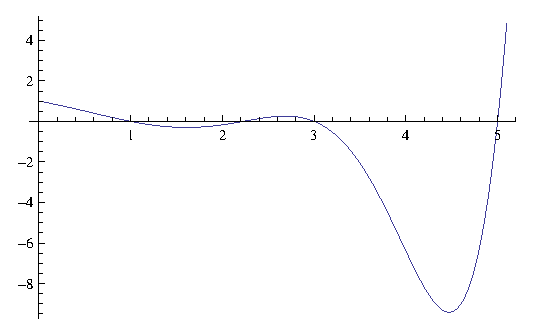
\includegraphics{PlotsRiemannH_gr1.eps}
	\caption{Plot of ${Z_1}( - s) = \frac{{\Gamma ( - \tfrac{s}{2})}}{{2\Gamma ( - s)}}{F_1}\left( { - \frac{s}{2},\frac{1}{2},\frac{1}{4}} \right)$ for $0 < s < 10$.}
\end{figure}
\noindent however, in the desired range $-\tfrac{1}{2}<\sigma<0$, and indeed all $\sigma$, one gets
\begin{figure}[H]
	\centering
		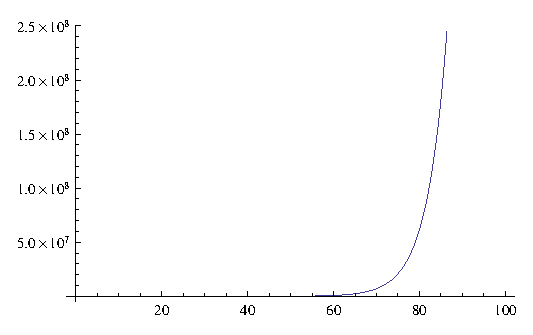
\includegraphics{PlotsRiemannH_gr2.eps}
	\caption{Plot of $\left| {{Z_1}( - \tfrac{1}{4} + it)} \right|$ for $0 < t <100$.}
\end{figure}
\noindent This is to be expected in view of \eqref{whynofluctuation}. Therefore, it raises the question on whether any such pair of functions $\varphi, \psi$ exists\footnote{If $Z_1(\sigma + it)$ grows like $\exp(|t|)t^a$, unless it starts at a negative value before it begins to grow, then $Z_1$ will only be positive and monotically increasing.} and if not, then statement (ii.b) of the theorem might be removed altogether.
%%%%%%%%%%%%%%%%%%%%%%%%%%%%%%%%%%%%%%%%%%%%%%%%%%%%%%%%%%%%%%%%%%%%%%%%%%%%%%%%%%%%%%%%%%%%%%%%%%%%%%%%%%%%%%%%%%%%%%%%%%%%%%%%%%%%%%%%%%%%%%%%%%%%%%
%%%%%%%%%%%%%%%%%%%%%%%%%%%%%%%%%%%%%%%%%%%%%%%%%%%%%%%%%%%%%%%%%%%%%%%%%%%%%%%%%%%%%%%%%%%%%%%%%%%%%%%%%%%%%%%%%%%%%%%%%%%%%%%%%%%%%%%%%%%%%%%%%%%%%%
\section{The bracketing condition and the simple zeros}
\noindent In the proof of the main theorem we have assumed, for simplicity, that the non-trivial zeros $\rho$ are all simple. However, it is not difficult to modify this argument to allow the possibility that some of the zeros are of higher order, say $\ell$ where $\ell \ge 2$. Let us denote the simple zeros by $\rho_1 = \rho$ and by $\rho_\ell$ the higher order zeros. In this case, the residues of $\rho_\ell$ are given by
\[
\kappa (\rho _\ell  ): = \frac{{\tau (\bar \chi )}}
{{\pi ^{1/2} }}\left( {\frac{b}
{{q^{1/2} }}} \right)^{\rho _\ell  } \frac{{\Gamma (1 - \rho _\ell  )}}
{{(\ell  - 1)!}}Z_2 (1 - \rho _\ell  )\mathop {\lim }\limits_{s \to \rho _\ell  } \frac{{d^{\ell  - 1} }}
{{ds^{\ell  - 1} }}\frac{{(s - \rho _\ell  )^\ell  }}
{{L(s,\bar \chi )}}
\]
We will denote the sum of these, perhaps non-existent, residues by
\begin{align} \label{higherorderzeros}
{\rm K}(\rho _\ell  ): = \sum\limits_{\rho _\ell  } {\kappa (\rho _\ell  )} .
\end{align}
We shall numerically investigate $\rm K$ and conclude that it is either very small or indeed zero.\\
Much like in \cite{dixit_1} and \cite{titchmarsh}, the convergence of the series involving $\rho$ on the right hand side of \eqref{higherorderzeros} cannot be proved in the ordinary sense, it can only be proved with the condition expressed in \eqref{dirichlet_bracketing_condition_eq}. That is, by the reasoning making the horizontal integrals of the contour tend to zero as $T \to \infty$, the series
\[
 - \frac{q}
{{\sqrt b }}\sqrt {\tau (\bar \chi )} {\rm K}(\rho _\ell  )
\]
converges only if we bracket the terms in such a way that two terms for which
\[
\left| {\gamma  - \gamma '} \right| < \exp ( - A_1 \gamma /\log \gamma ) + \exp ( - A_1 \gamma '/\log \gamma ')
\]
are included in the same bracket. On average, the zeros are father apart than this (the average spacing between zeros is $2\pi / \log \gamma_n$) and therefore according to \cite{titchmarsh} it is quite likely that the convergence is true without any bracketing, or according to \cite{hardy_littlewood} the series is not just merely convergent but in fact rapidly convergent. Numerical analysis to appreciate these claims will be provided shortly.\\
Dixit \cite{dixit_1} has suggested the following: \eqref{Hardy-Littlewood-Ramanujan} may be written as
\begin{align} \label{dixit_equivalent}
\sqrt a \sum\limits_{n = 1}^\infty  {\frac{{\mu (n)}}
{n}e^{ - a^2 /n^2 } }  - \frac{1}
{{2\sqrt a }}\sum\limits_\rho  {a^\rho  \frac{{\Gamma (\tfrac{{1 - \rho }}
{2})}}
{{\zeta '(\rho )}}}  = \sqrt b \sum\limits_{n = 1}^\infty  {\frac{{\mu (n)}}
{n}e^{ - b^2 /n^2 } }  - \frac{1}
{{2\sqrt b }}\sum\limits_\rho  {b^\rho  \frac{{\Gamma (\tfrac{{1 - \rho }}
{2})}}
{{\zeta '(\rho )}}}.
\end{align}
Let us denote the left hand side by $F(a)$ and the right hand side by $F(b)$. Since \eqref{hardy_littlewood_original_eq} is of the form $F(a)=F(b)$ for $ab = \pi$ then it natural to ask if there exists an integral representation involving the $\Xi(t)$ function
\[
\Xi (t): = \xi \left( {\frac{1}
{2} + it} \right),\quad \xi (s): = \frac{1}
{2}s(s - 1)\pi ^{ - s/2} \Gamma \left( {\frac{s}
{2}} \right)\zeta (s)
\]
of the form
\[
F(a): = \int_0^\infty  {f\left( {\frac{t}
{2}} \right)\Xi \left( {\frac{t}
{2}} \right)\cos (\mu (a)t)dt} 
\]
where $\mu$ is a real function of $a$ and $f(t)=\phi(it)\phi(-it)$ where $\phi$ is analytic in $t$ as a function of a real variable. This integral representation is of some prominence in the work of Ramanujan \cite{ramanujan_32} and Hardy \cite{hardy}, \cite{titchmarsh} who used it to prove that $\zeta(s)$ has infinitely many zeros on the critical line. Indeed, formulae of the type $F(a)=F(b)$ with the constraint $ab = k$ where $k$ is a constant results from considering such integral representations.\\
Consequently, it is reasonable to expect that if such an integral representation did exist and certain criteria are met or bypassed (e.g. the convergence of such an integral) then this might \cite{dixit_1} throw some light into the convergence of sums involving $\rho$ without consideration to the bracketing.\\
Unfortunately, with other approaches \cite{hardy_littlewood} based on the assumption of the Riemann hypothesis, the convergence of the series without bracketing seems to be out of reach.
(\textcolor{red}{From here until the end, I need to seriously fix that. For the moment, you can ignore.}) Let us now go back to the Hardy-Littlewood formula. If we write the sum involving $a$ of the left hand side as $F(a)$ we see that a Taylor expansion yields
\begin{align} \label{derivative_minus_even_integers}
  F(a) &: = \sum\limits_{n = 1}^\infty  {\frac{{\mu (n)}}
{n}e^{ - (a/n)^2 } } = \sum\limits_{k = 1}^\infty  {\frac{{( - 1)^k }}
{{k!}}\frac{{a^{2k} }}
{{\zeta (2k + 1)}}}  = \frac{1}
{{2\sqrt \pi  }}\sum\limits_{k = 1}^\infty  {b^{ - 2k} \frac{{\Gamma (\tfrac{1}
{2} + k)}}
{{\zeta '( - 2k)}}}   
\end{align}
where we have used 
\[
\zeta '( - 2k) = \frac{{( - 1)^k \zeta (2k + 1)(2k)!}}
{{2^{2k + 1} \pi ^{2k} }},\quad \frac{{(2k)!}}
{{2^{2k + 1} k!}} = \frac{{\Gamma (\tfrac{1}
{2} + k)}}
{{2\sqrt \pi  }}
\]
for $k=1,2,3, \cdots$. Furthermore, by symmetry we see that
\[
\frac{1}
{{\sqrt a }}\sum\limits_\rho  {\frac{{a^\rho  \Gamma (\tfrac{1}
{2} - \tfrac{1}
{2}\rho )}}
{{\zeta '(\rho )}}}  + \frac{1}
{{\sqrt b }}\sum\limits_\rho  {\frac{{b^\rho  \Gamma (\tfrac{1}
{2} - \tfrac{1}
{2}\rho )}}
{{\zeta '(\rho )}}}  = 0.
\]
Using \eqref{derivative_minus_even_integers} we can write
\[
\sqrt b \sum\limits_{n = 1}^\infty  {\frac{{\mu (n)}}
{n}e^{ - (b/n)^2 } }  = \frac{1}
{{2\sqrt b }}\sum\limits_\rho  {\frac{{b^\rho  \Gamma (\tfrac{1}
{2} - \tfrac{1}
{2}\rho )}}
{{\zeta '(\rho )}}}  + \sqrt a \frac{1}
{{2\sqrt \pi  }}\sum\limits_{k = 1}^\infty  {b^{ - 2k} \frac{{\Gamma (\tfrac{1}
{2} + k)}}
{{\zeta '( - 2k)}}}. 
\]
If we take $a=\pi$ so that $b=1$ then
\begin{align} \label{0_7}
  \sum\limits_{n = 1}^\infty  {\frac{{\mu (n)}}
{n}e^{ - (1/n)^2 } } &= \frac{1}
{2}\sum\limits_\rho  {\frac{{\Gamma (\tfrac{1}
{2} - \tfrac{1}
{2}\rho )}}
{{\zeta '(\rho )}}}  + \sqrt \pi  \sum\limits_{k = 1}^\infty  {\frac{{( - 1)^k }}
{{k!}}\frac{{\pi ^{2k} }}
{{\zeta (1 + 2k)}}} \\
  \label{0_8} &= \frac{1}
{2}\sum\limits_\rho  {\frac{{\Gamma (\tfrac{1}
{2} - \tfrac{1}
{2}\rho )}}
{{\zeta '(\rho )}}}  + \frac{1}
{2}\sum\limits_{k = 1}^\infty  {\frac{{\Gamma (\tfrac{1}
{2} + k)}}
{{\zeta '( - 2k)}}}   
\end{align}
If higher order zeros $\rho_\ell$ exist then we would have to add ${\rm K}(\rho _\ell)$ to the right hand side of \eqref{0_7} and \eqref{0_8}. The LHS, that is, the sum involving the M\"{o}bius function oscillates erratically. For $n=100$ we have $\sum\nolimits_{n = 1}^{100} {\tfrac{{\mu (n)}}{n}e^{ - (1/n^2 )} }  \approx  - 0.4494055445$ and the following plot
\begin{figure}[H]
%	\centering
		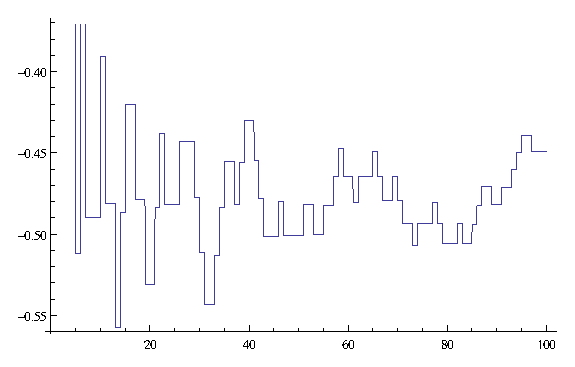
\includegraphics[scale=0.96]{MoebiusNov100and1000and10000_gr1.eps}
		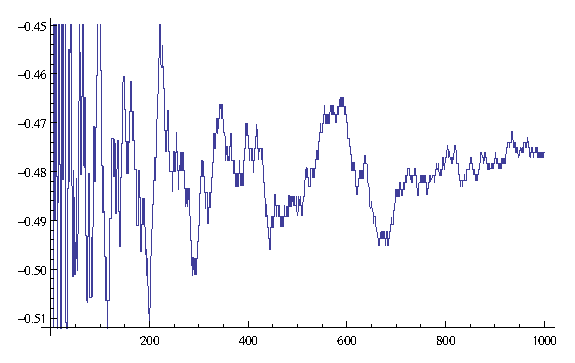
\includegraphics[scale=0.96]{MoebiusNov100and1000and10000_gr2.eps}
	\caption{Plot of $\sum\nolimits_{n = 1}^{x} {\tfrac{{\mu (n)}}{n}e^{ - (1/n^2 )} }$ for $1 \le x \le 100$.}
	\caption{Plot of $\sum\nolimits_{n = 1}^{x} {\tfrac{{\mu (n)}}{n}e^{ - (1/n^2 )} }$ for $1 \le x \le 1000$.}
\end{figure}
\noindent so that and for $n=1000$ we have $\sum\nolimits_{n = 1}^{1000} {\tfrac{{\mu (n)}}{n}e^{ - (1/n^2 )} }  \approx  - 0.4761219362$ and if we take $n=100000$ then 
\begin{align} \label{numerical_sum_100000_moebius}
\sum\nolimits_{n = 1}^{10000} {\tfrac{{\mu (n)}}{n}e^{ - (1/n^2 )} }  \approx  - 0.4826165005
\end{align}
\noindent and
\begin{figure}[H]
	\centering
		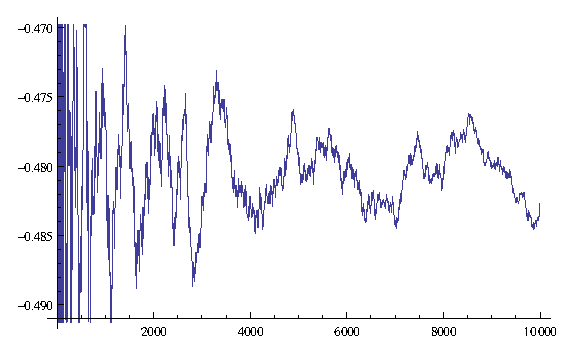
\includegraphics{MoebiusNov100and1000and10000_gr3.eps}
	\caption{Plot of $\sum\nolimits_{n = 1}^{x} {\tfrac{{\mu (n)}}{n}e^{ - (1/n^2 )} }$ for $1 \le x \le 10000$.}
\end{figure}
\noindent The sum of the first hundred pairs of zeros $\rho$ (which of course are simple and located on the critical line) yields
\begin{align} \label{numerical_sum_100_rhos}
\frac{1}
{2}\sum\limits_\rho  {\frac{{\Gamma (\tfrac{1}
{2} - \tfrac{1}
{2}\rho )}}
{{\zeta '(\rho )}}}  \approx 0.000028488145133.
\end{align}
\noindent The sum over $\zeta'(-2k)$ is more difficult and it also fluctuates.% The plot is initially very large in magnitude but eventually settles down. A similar computation as the one above shows that for $n=10$ we have $\tfrac{1}{2}\sum\nolimits_{k = 1}^x {\tfrac{{\Gamma (\tfrac{1}{2} + k)}}{{\zeta '( - 2k)}}} \approx 2072.090288$ and the following plot
%\begin{figure}[H]
%	\centering
%		\includegraphics{GammZetaDerivative10100100010000_gr1.eps}
%	\caption{Plot of $\tfrac{1}{2}\sum\nolimits_{k = 1}^x {\tfrac{{\Gamma (\tfrac{1}{2} + k)}}{{\zeta '( - 2k)}}}$ for $1 \le x \le 10$.}
%\end{figure}
%for $n=1000$ we have 
%\begin{align} \label{numerical_sum_1000_gamma_der_zeta}
%\tfrac{1}{2}\sum\nolimits_{k = 1}^x {\tfrac{{\Gamma (\tfrac{1}{2} + k)}}{{\zeta '( - 2k)}}} \approx -0.480562288941
%\end{align}
%\noindent and
%\begin{figure}[H]
%	\centering
%		\includegraphics{GammZetaDerivative10100100010000_gr2.eps}
%	\caption{Plot of $\tfrac{1}{2}\sum\nolimits_{k = 1}^x {\tfrac{{\Gamma (\tfrac{1}{2} + k)}}{{\zeta '( - 2k)}}}$ for $1 \le x \le 100$.}
%\end{figure}
If we take $n=1000$ and $n=10'000 $then $\tfrac{1}{2}\sum\nolimits_{k = 1}^x {\tfrac{{\Gamma (\tfrac{1}{2} + k)}}{{\zeta '( - 2k)}}}$ is seen to be
\begin{figure}[H]
		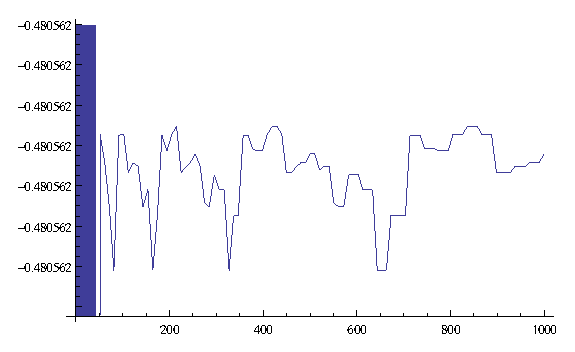
\includegraphics[scale=0.96]{GammZetaDerivative10100100010000_gr3.eps}
		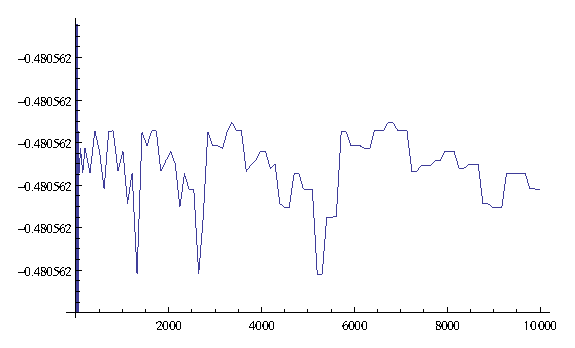
\includegraphics[scale=0.96]{GammZetaDerivative10100100010000_gr4.eps}
	\caption{Plot of $\tfrac{1}{2}\sum\nolimits_{k = 1}^x {\tfrac{{\Gamma (\tfrac{1}{2} + k)}}{{\zeta '( - 2k)}}}$ for $1 \le x \le 1000$ and $1 \le x \le 10000$.}
\end{figure}
\noindent Consequently, if we use the approximations \eqref{numerical_sum_100000_moebius}, \eqref{numerical_sum_100_rhos} and \eqref{numerical_sum_1000_gamma_der_zeta} we see that the LHS of \eqref{0_8} is $-0.4826165005$ whereas its RHS is $-0.48053380079607$. The difference is approximately, $-0.002082699747$.\\ 
Arguably, much can be done to improve these modest approximations, however the disagreement between both sides might indicate that $\rm{K}$ might not be zero in order to compensate this difference and therefore higher order zeros might exist.
%%%%%%%%%%%%%%%%%%%%%%%%%%%%%%%%%%%%%%%%%%%%%%%%%%%%%%%%%%%%%%%%%%%%%%%%%%%%%%%%%%%%%%%%%%%%%%%%%%%%%%%%%%%%%%%%%%%%%%%%%%%%%%%%%%%%%%%%%%%%%%%%%%%%%%
%%%%%%%%%%%%%%%%%%%%%%%%%%%%%%%%%%%%%%%%%%%%%%%%%%%%%%%%%%%%%%%%%%%%%%%%%%%%%%%%%%%%%%%%%%%%%%%%%%%%%%%%%%%%%%%%%%%%%%%%%%%%%%%%%%%%%%%%%%%%%%%%%%%%%%
\subsection{Conclusion and future work}
\noindent As it has been discussed, the most satisfying aspect of these explicit formulae would be to remove the bracketing condition. However, this \textcolor{red}{seems} to belong to the new generation of questions that one asks themselves once the issue of the Riemann hypothesis is settled.\\\\
There are however, different ways of extending this work. This can be done as follows.
\begin{enumerate}
\item[(a)] We could consider other $L$ functions. For instance, if we do the same analysis with the Dedekind zeta function over a field $K$ then
\begin{align}
  {a^{{r_1}/2 + {r_2}}}\sum\limits_\mathfrak{a} {\frac{{{\mu _K}(\mathfrak{a})}}{{N(\mathfrak{a})}}\mathcal{Q}\left( {\frac{{{a^{{r_1} + 2{r_2}}}}}{{N(\mathfrak{a})}}} \right)}  &- {2^{{r_2}}}{b^{{r_1}/2 + {r_2}}}{\left| {{\Delta _K}} \right|^{1/2}}\sum\limits_\mathfrak{a} {\frac{{{\mu _K}(\mathfrak{a})}}{{N(\mathfrak{a})}}\mathcal{Q}\left( {\frac{{{2^{2{r_2}}}{b^{{r_1} + 2{r_2}}}\left| {{\Delta _K}} \right|}}{{N(\mathfrak{a})}}} \right)}  \nonumber \\
   &= \frac{1}{{{a^{{r_1}/2 + {r_2}}}}}\sum\limits_{{\rho _K}} {{a^{({r_1} + 2{r_2}){\rho _K}}}\frac{{{\Gamma ^{{r_1}}}(\tfrac{{1 - {\rho _K}}}{2}){\Gamma ^{{r_2}}}(1 - {\rho _K})}}{{{\zeta _K}'({\rho _K})}}}  \nonumber \\
	&- {a^{{r_1}/2}}{a^{{r_2}}}R_K(a). \nonumber 
\end{align}
where the quantities $\mathcal{Q}$ and $R_K$ are computable, $\Delta_K$ is the discriminant of the field $K$ \textcolor{red}{etc}... Also, if we take the Hasse-Weil zeta function instead then
\begin{align}
  \frac{{N(E)}}{{{{(2\pi )}^2}}}\sum\limits_{n = 1}^\infty  {\frac{{{a_E}(n)}}{{{n^2}}}{e^{ - 1/({b^2}n)}}}  &- \frac{1}{{{w_E}}}\sum\limits_{n = 1}^\infty  {\frac{{{\mathfrak{u}_E}(n)}}{{{n^2}}}{e^{ - 1/({a^2}n)}}}  \nonumber \\
   &= \sum\limits_{{\rho _E}} {{a^2}{b^{2 - 2{\rho _E}}}\frac{{\Gamma (2 - {\rho _E})}}{{L'({\rho _E},s)}}}  + {a^2}\mathop {\lim }\limits_{s \to 1} \frac{{{{(s - 1)}^{\operatorname{rank} (E(\Q))}}}}{{L(E,s)}}, \nonumber 
\end{align}
where $E$ is an elliptic curve over $\Q$ defined by
\[E:{y^2} = {x^3} + ax + b,\]
where $a,b \in \Z$ satisfy $\Delta = -16(4a^3+27b^2) \ne 0$ \textcolor{red}{etc}... This has the advantage of incorporating algebraic information as well as arithmetical information.
\item[(b)] Other arithemtical functions may be studied, not just the M\"{o}bius function. For instance, repeating a similar analysis for Liouville's $\lambda$ function defined by $\lambda(n)=(-1)^{r}$ if $n$ has $r$ prime factors, a factor of degree $k$ being counted $k$ times, then
\begin{align}
\sum\limits_{n = 1}^\infty  {\lambda (n)e^{ - an} }  - \sum\limits_{n = 1}^\infty  {\frac{1}
{n}\sum\limits_{m = 1}^\infty  {\frac{{\mu (m)}}
{m}} F_{\lambda,2}  (bmn^2)}  &= \sum\limits_{\rho \in \mathcal{B}}  {a^{ - \rho } \Gamma (\rho )\frac{{\zeta (2\rho )}}
{{\zeta '(\rho )}}}  + \frac{1}
{2}a^{1/2} \frac{{\pi ^{1/2} }}
{{\zeta (\tfrac{1}
{2})}} + 1 \nonumber \\
& = - \sum\limits_{\rho \in \mathcal{B}}  {b^\rho  \frac{{\Gamma (\tfrac{1}
{2} - \rho )\Gamma (\tfrac{1}
{2}\rho )}}
{{\Gamma (\tfrac{1}
{2} - \tfrac{1}
{2}\rho )}}\frac{{\zeta (1 - 2\rho )}}
{{\zeta '(1 - \rho )}}} + \frac{\sqrt{b}}{2\zeta(\tfrac{1}{2})} +1, \nonumber
\end{align}
where $ab = \pi$ with $b \ge 2$ and 
\[
F_{\lambda ,2} (x) = \frac{1}
{{\sqrt x \sqrt {4 + x^{ - 2} } }}\left( {\sqrt {2 + \sqrt {4 + x^{ - 2} } }  + \sqrt 2 (4 + x^{ - 2} )^{1/4} \sin \left[ {\frac{1}
{2}\operatorname{arccot} (2x)} \right]} \right).
\]
See \cite{kuhnrobles2} for an analysis on other arithemtical functions such as the Euler totient function, von Mangoldt function etc.
\item[(c)] Other transforms \cite{hardy_titchmarsh}: both the cosine and sine transformations are special cases of the more general Hankel transform
\[f(x) = \int_0^\infty  {\sqrt {xy} {J_\nu }(xy)g(y)dy} ,\quad g(x) = \int_0^\infty  {\sqrt {xy} {J_\nu }(xy)f(y)dy}, \]
where ${J_\nu }$ is the Bessel function of order $\nu \ge -\tfrac{1}{2}$. The cosine and sine cases are the cases in which $\nu = -\tfrac{1}{2}$ and $n = \tfrac{1}{2}$.
\end{enumerate}
%%%%%%%%%%%%%%%%%%%%%%%%%%%%%%%%%%%%%%%%%%%%%%%%%%%%%%%%%%%%%%%%%%%%%%%%%%%%%%%%%%%%%%%%%%%%%%%%%%%%%%%%%%%%%%%%%%%%%%%%%%%%%%%%%%%%%%%%%%%%%%%%%%%%%%
%%%%%%%%%%%%%%%%%%%%%%%%%%%%%%%%%%%%%%%%%%%%%%%%%%%%%%%%%%%%%%%%%%%%%%%%%%%%%%%%%%%%%%%%%%%%%%%%%%%%%%%%%%%%%%%%%%%%%%%%%%%%%%%%%%%%%%%%%%%%%%%%%%%%%%
\subsection{References}
\begin{thebibliography}{99}

	\bibitem{abyz} S.~Ahlgren, B.~C.~Berndt, A.~J.~Yee and A.~Zaharescu \emph{Integrals of Eisenstein Series and Derivatives of $L$-functions}, CiteSeerX 10.1.1.128.5078.
	
	%\bibitem{apostol} T.~M.~Apostol, \emph{Introduction to Analytic Number Theory}, Springer Verlag, 1976.
	
	%\bibitem{berndt} B.~C.~Berndt, \emph{Ramanujan Reaches His Hand From His Grave To Snatch Your Theorems From You}, Asia Pacific Mathematics Newsletter, April 2011, Volume 1 No 2.
	
	\bibitem{davenport} H.~Davenport, \emph{Multiplicative Number Theory}, Markham Publishing Company, 1967.
	
	\bibitem{dixit_1} A.~Dixit, \emph{Character Analogues of Ramanujan type integrals involving the Riemann $\Xi$-function}, Pacific Journal of Mathematics, Vol. 255 (2012), No. 2, 317?48.
	
	\bibitem{dixit_2} A.~Dixit, \emph{Analogues of the general theta transformation formula}, Proceedings of the Royal Society of Edinburg, \textbf{143A}, 371-399, 2013.
	
	\bibitem{dixit_3} A.~Dixit, A.~Roy, A.~Zaharescu \emph{Analogues of the general theta transformation formula, II}, to appear, 2013.
	
	\bibitem{dixit_4} A.~Dixit, A.~Roy, A.~Zaharescu \emph{Ramanujan-Hardy-Littlewood-Riesz phenomena for Hecke forms}, to appear, 2013.
	
	\bibitem{hardy} G.~H.~Hardy, \emph{Sur les z\'eros de la fonction $\zeta(s)$ de Riemann}, 1914 \textit{Comptes Rendus}, \textbf{158}, 1012-14.
	
	\bibitem{hardy_littlewood} G.~H.~Hardy and J.~E.~Littlewood, \emph{Contributions to the Theory of the Riemann Zeta-Function and the Theory of the Distribution of Primes}, 1918 Acta Mathematica 41, 119-86.
	
	\bibitem{hardy_titchmarsh} G.~H.~Hardy and E.~C.~Titchmarsh, \emph{Self-reciprocal functions}, The Quarterly Journal of Mathematics, vol. os-1, no. 1, pp. 196-231
	
	\bibitem{hoheisel_3} G.~Hoheisel, \emph{\"{U}ber das Verhalten des reziproken Wertes der Riemannschen Zetafunktion}, Sitzungsber. Preuss. Akad. Wiss. (1929), 219-23.
	
	%\bibitem{iwaniec_kowalski} H.~Iwaniec and E.~Kowalski, \emph{Analytic Number Theory}, American Mathematical Society, Colloquium Publications Volume 53, Prodivence, Rhode Island, 2004.
	
	\bibitem{kuhnrobles2} P.~K\"{u}hn and N.~Robles, \emph{Arithmetical functions and their explicit formulae through combinations of functional equations of $\zeta(s)$}, in preparation
	
	\bibitem{landau_8} E.~Landau, \emph{\"{U}ber die Hardysche Entdeckung unendlich vieler Nullstellen der Zetafunktion mit reellem Teil $\tfrac{1}{2}$}, M.A. 76 (1915), 212-43.
	
	\bibitem{landau_18} E.~Landau, \emph{\"{U}ber die Zetafunktion und die Hadamardsche Theorie der ganzen Funktionen}, M.Z. 26 (1927), 170-5.
	
	\bibitem{littlewood_jan_12} J.~E.~Littlewood, \emph{Quelques cons\'{e}quences de l'hypoth\`{e}se que la fonction $\zeta(s)$ de Riemann n'a pas de z\'{e}ros dans le demi-plan $\operatorname{Re}(s) > \tfrac{1}{2}$}, Comptes Rendus, S\'{e}ance du 29 Janvier 1912.
	
	%\bibitem{murty} M.~R.~Murty, \emph{Problems in Analytic Number Theory}, Springer Verlag, 2001.
	
	\bibitem{ramanujan_32} S.~Ramanujan, \emph{New expressions for Riemann's functions $\xi(s)$ and $\Xi(t)$}, Quart. J. Math, \textbf{46}, (1915), 253-260.
	
	\bibitem{riesz} M.~Riesz, \emph{On the Riemann hypothesis}, Acta Mathematica, \textbf{40}, December 20th 1916.
	
	\bibitem{titchmarsh4} E.~C.~Titchmarsh, \emph{On an inequality satisfied by the zeta-function of Riemann}, P. L. M. S. (2) 28 (1928), 70-80.
	
	\bibitem{titchmarsh} E.~C.~Titchmarsh, \emph{Theory of Fourier Integrals}, Second Edition, Oxford University Press 1948.
	
	\bibitem{titchmarsh} E.~C.~Titchmarsh, \emph{The Theory of the Riemann Zeta-Function}, Second Edition revised D.~R.~Heath-Brown, Oxford University Press 1986.
	
	\bibitem{valiron} G.~Valiron, \emph{Sur les fonctions enti\`{e}res d'ordre nul et d'ordre fini}, Annales de Toulouse (3), 5 (1914), 117-257.
	
	%\bibitem{whittaker} E.~T.~Whittaker and G.~N.~Watson, \emph{A Course in Modern Analysis}, Cambridge University Press 1962.
	
\end{thebibliography}
\end{document}


By the Riemann - von Mangoldt formula, the number of zeros $N(T)$ up to height $T$ inside the critical strip is
\[N(T) = \frac{T}{{2\pi }}\log \frac{T}{{2\pi }} - \frac{T}{{2\pi }} + O(\log T).\]
This implies that if $\gamma_n$ is the $n$-th ordinate, then the average spacing between zeros is given by
\[\frac{{2\pi }}{{\log {\gamma _n}}}.\]
Thus the zeros are, on the average, much futher apart than 